\documentclass[dvipdfmx, twocolumn]{jsarticle}

\usepackage[version=3]{mhchem}
\usepackage{amsmath}
\usepackage[siunitx]{circuitikz}
\usepackage{graphicx}
\usepackage{here}

\setlength\parindent{0pt}

\begin{document}
\title{20 高電圧実験  考察報告書 }
\author{電子情報工学科 03-190449 堀 紡希}
\date{\ 11月5日}
\maketitle

\section{実験結果}
\subsection*{A. 交流高電圧}

\subsubsection*{A1. 電源回路}

略

\subsubsection*{A2. 球ギャップの火花電圧}

\begin{figure}[H]
\begin{center}
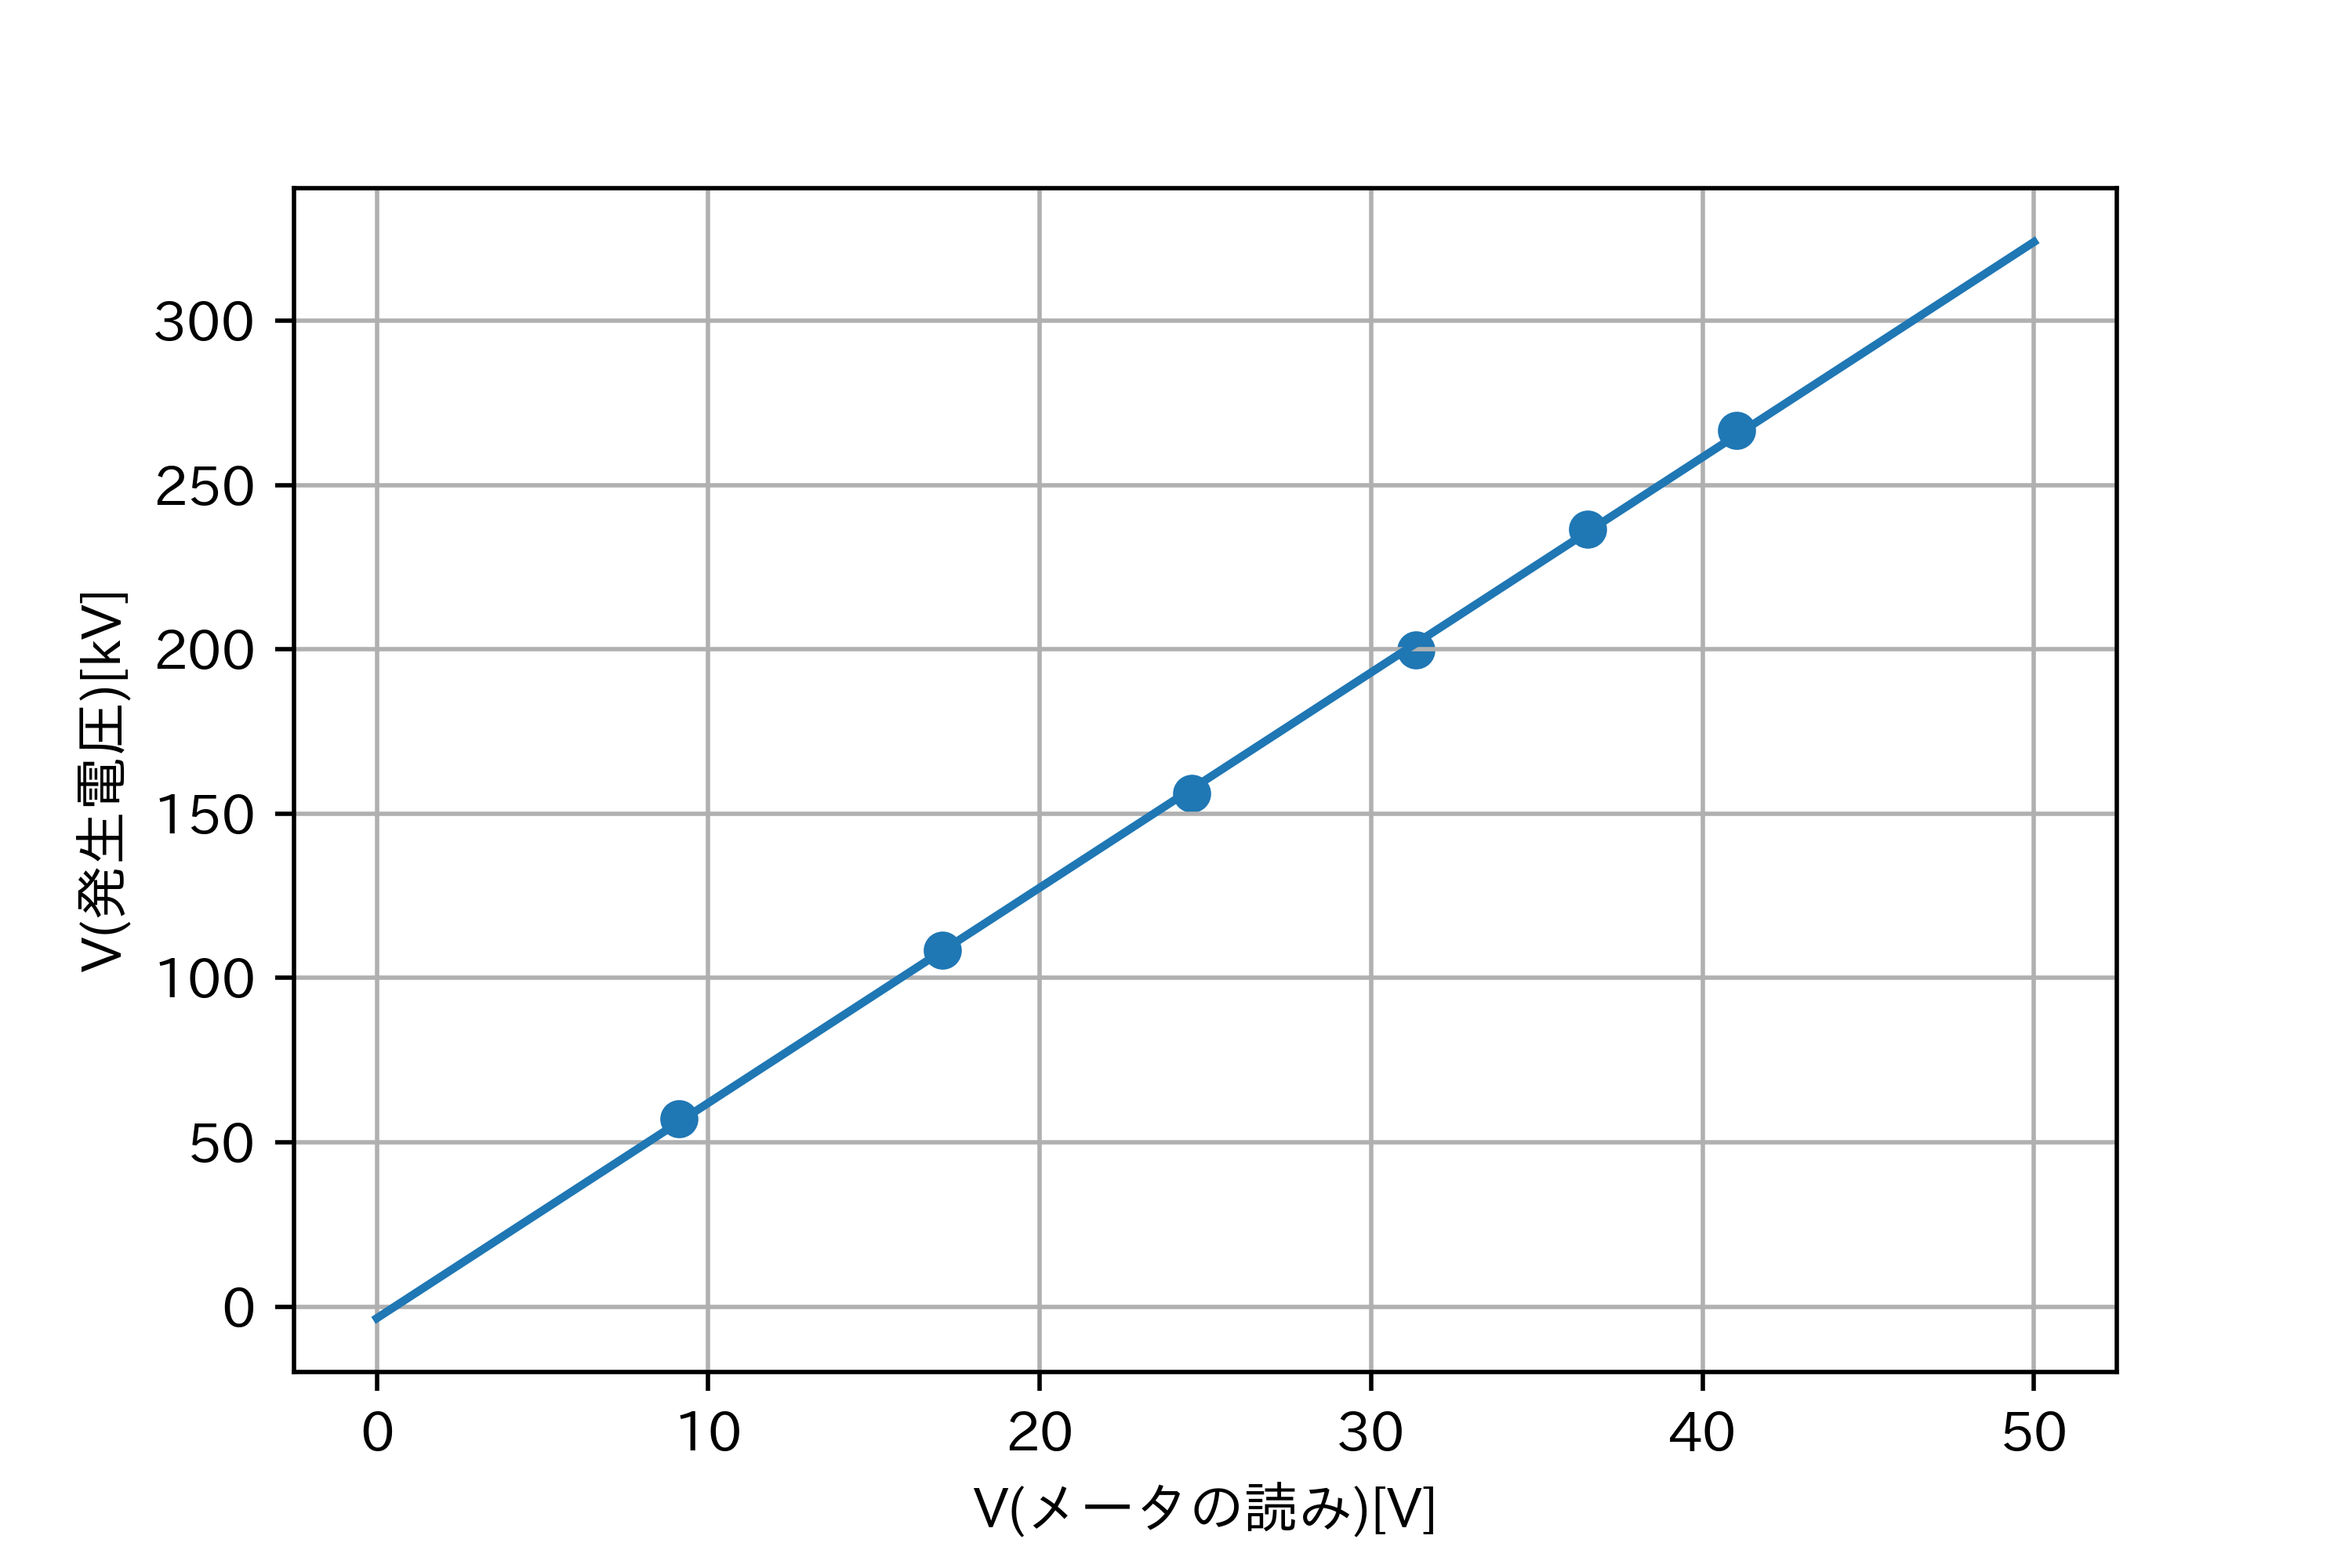
\includegraphics[scale = 0.5]{A2.png}
\caption{発生電圧の校正曲線}
\end{center}
\end{figure}
およそ$\delta$ = 0.97で補正し、
一次側電圧を$V_{1}$、発生電圧を$V_{2}$とすると、
$V_{2} = 6.548\times V_{1}-3.48$
という関係が得られた。
\subsubsection*{A3. 針-平板ギャップの火花特性}
\begin{figure}[H]
\begin{center}
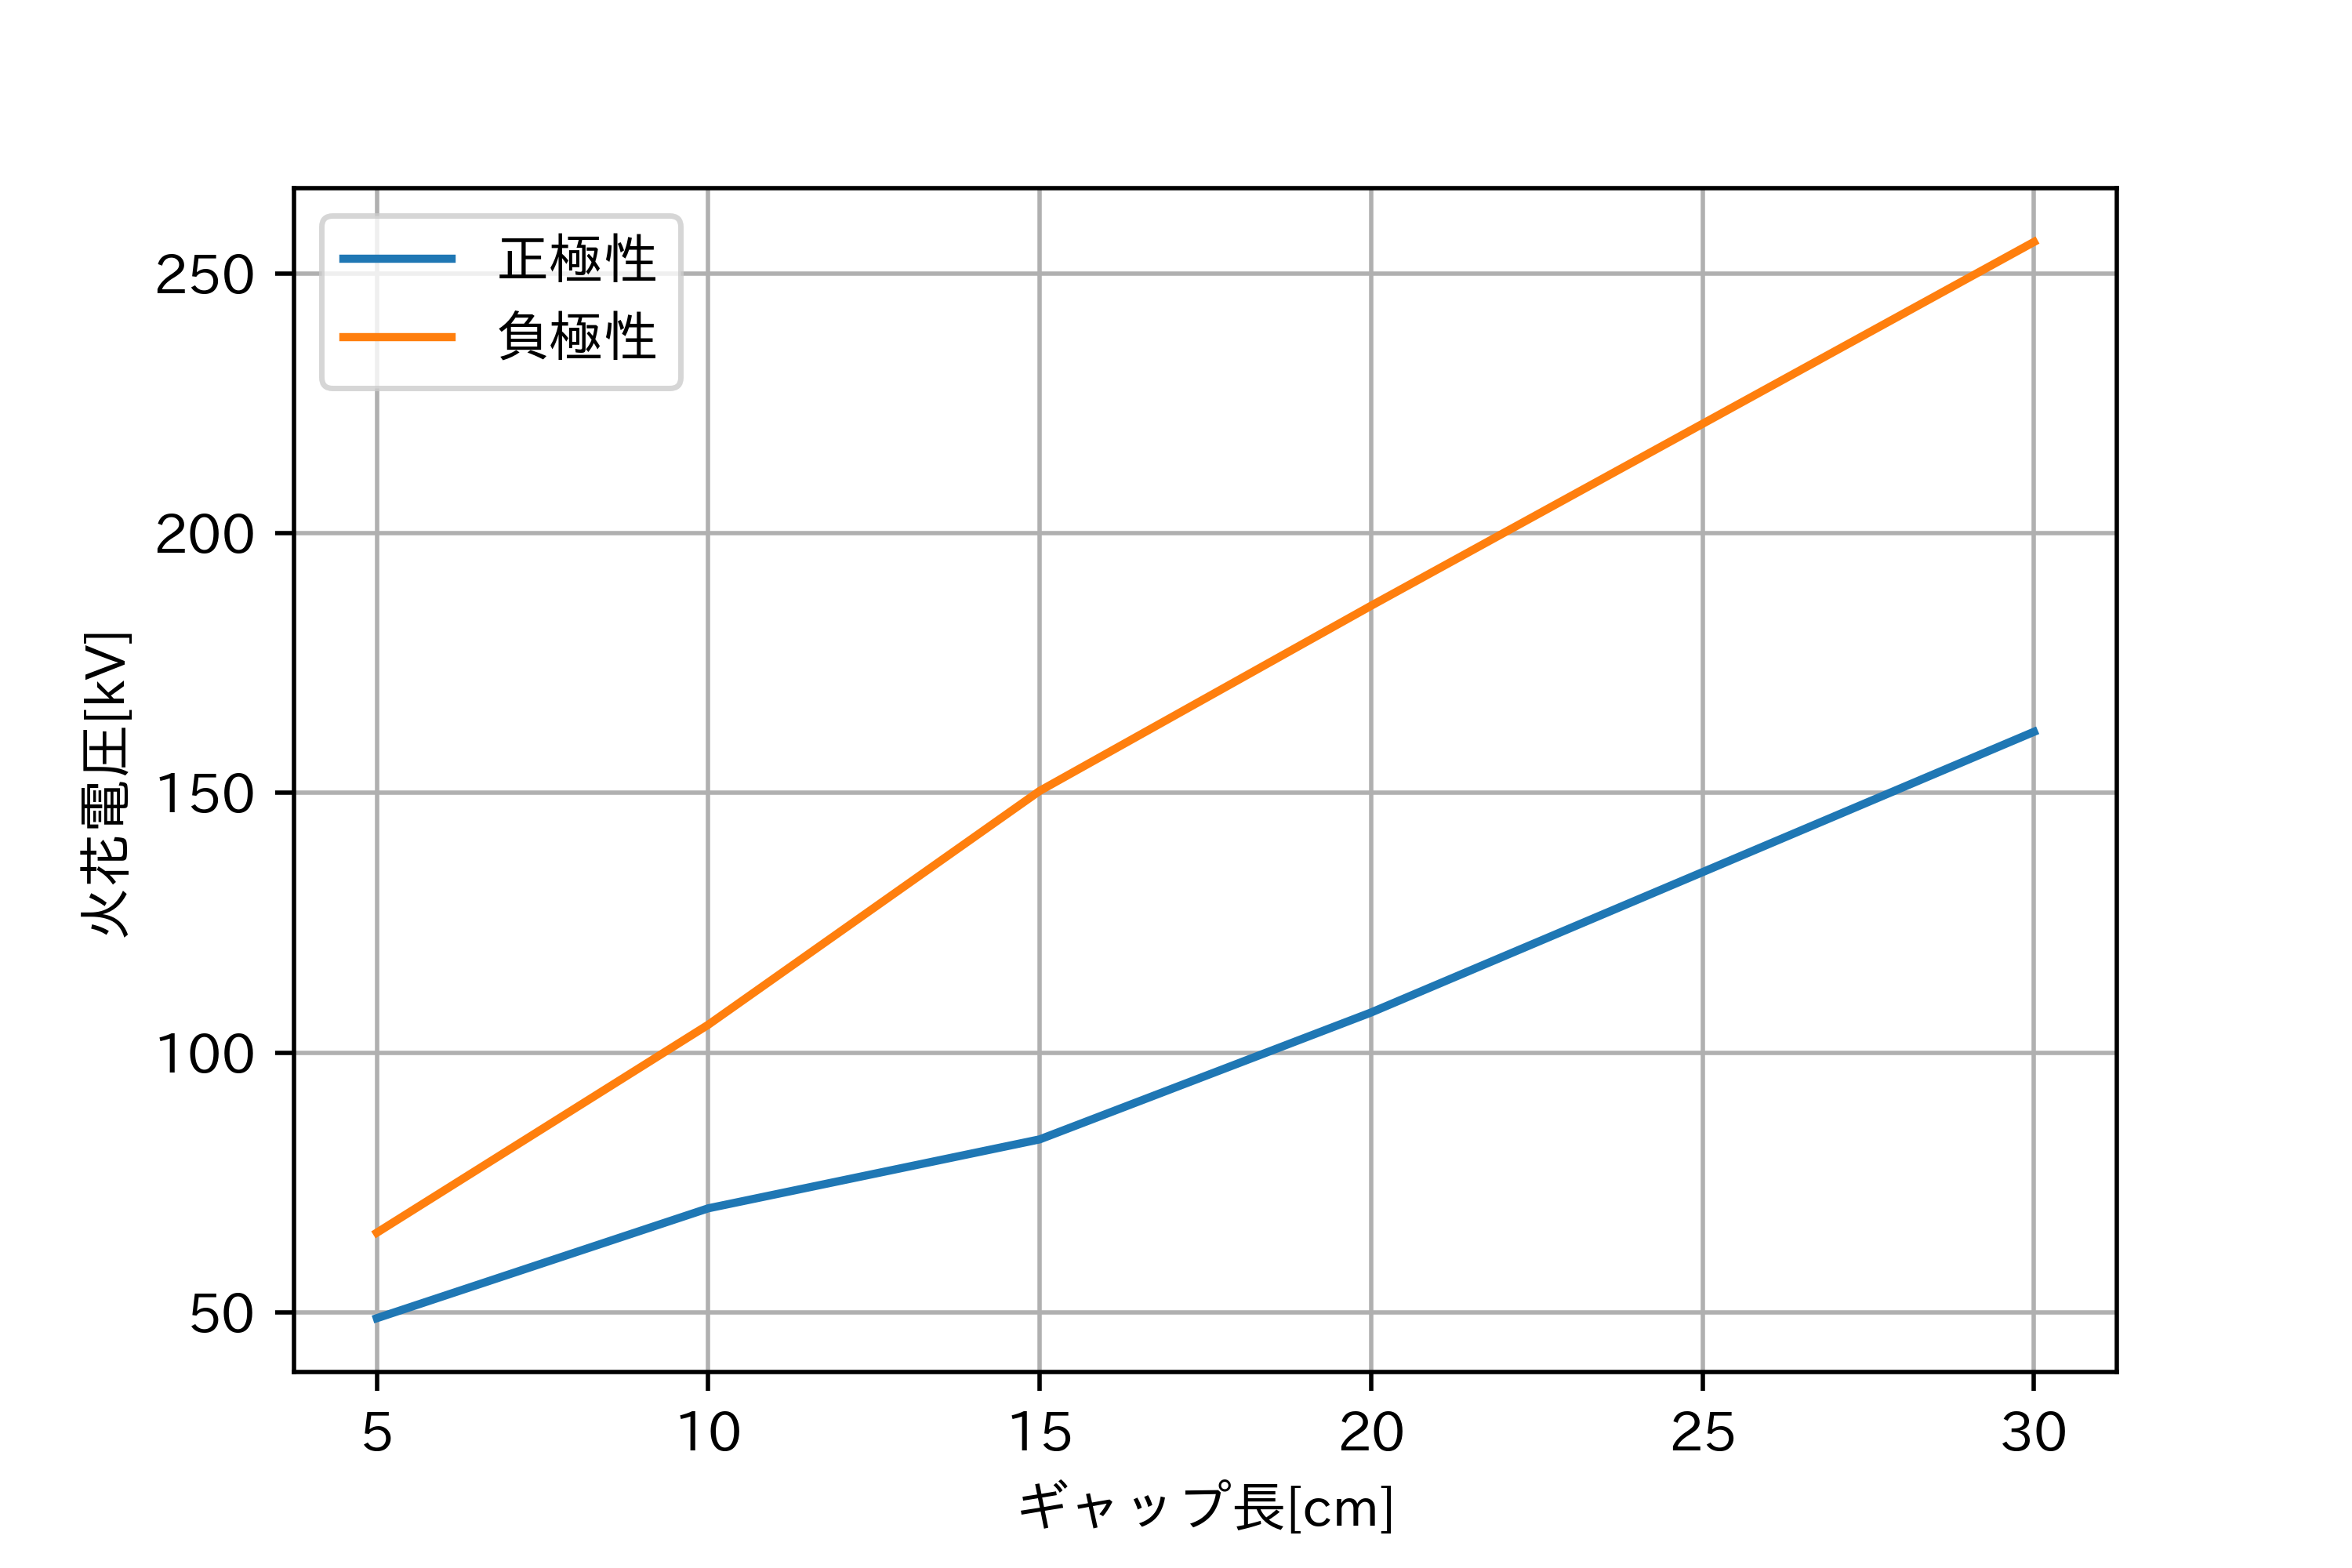
\includegraphics[scale = 0.5]{A3.png}
\caption{針-平板ギャップの火花特性}
\end{center}
\end{figure}
負極性では正極性の1.5倍ほどの火花電圧になっていることがわかる。

\subsubsection*{A4. 六フッ化イオウ (SF$_{6}$)中の火花電圧}

\begin{figure}[H]
\begin{center}
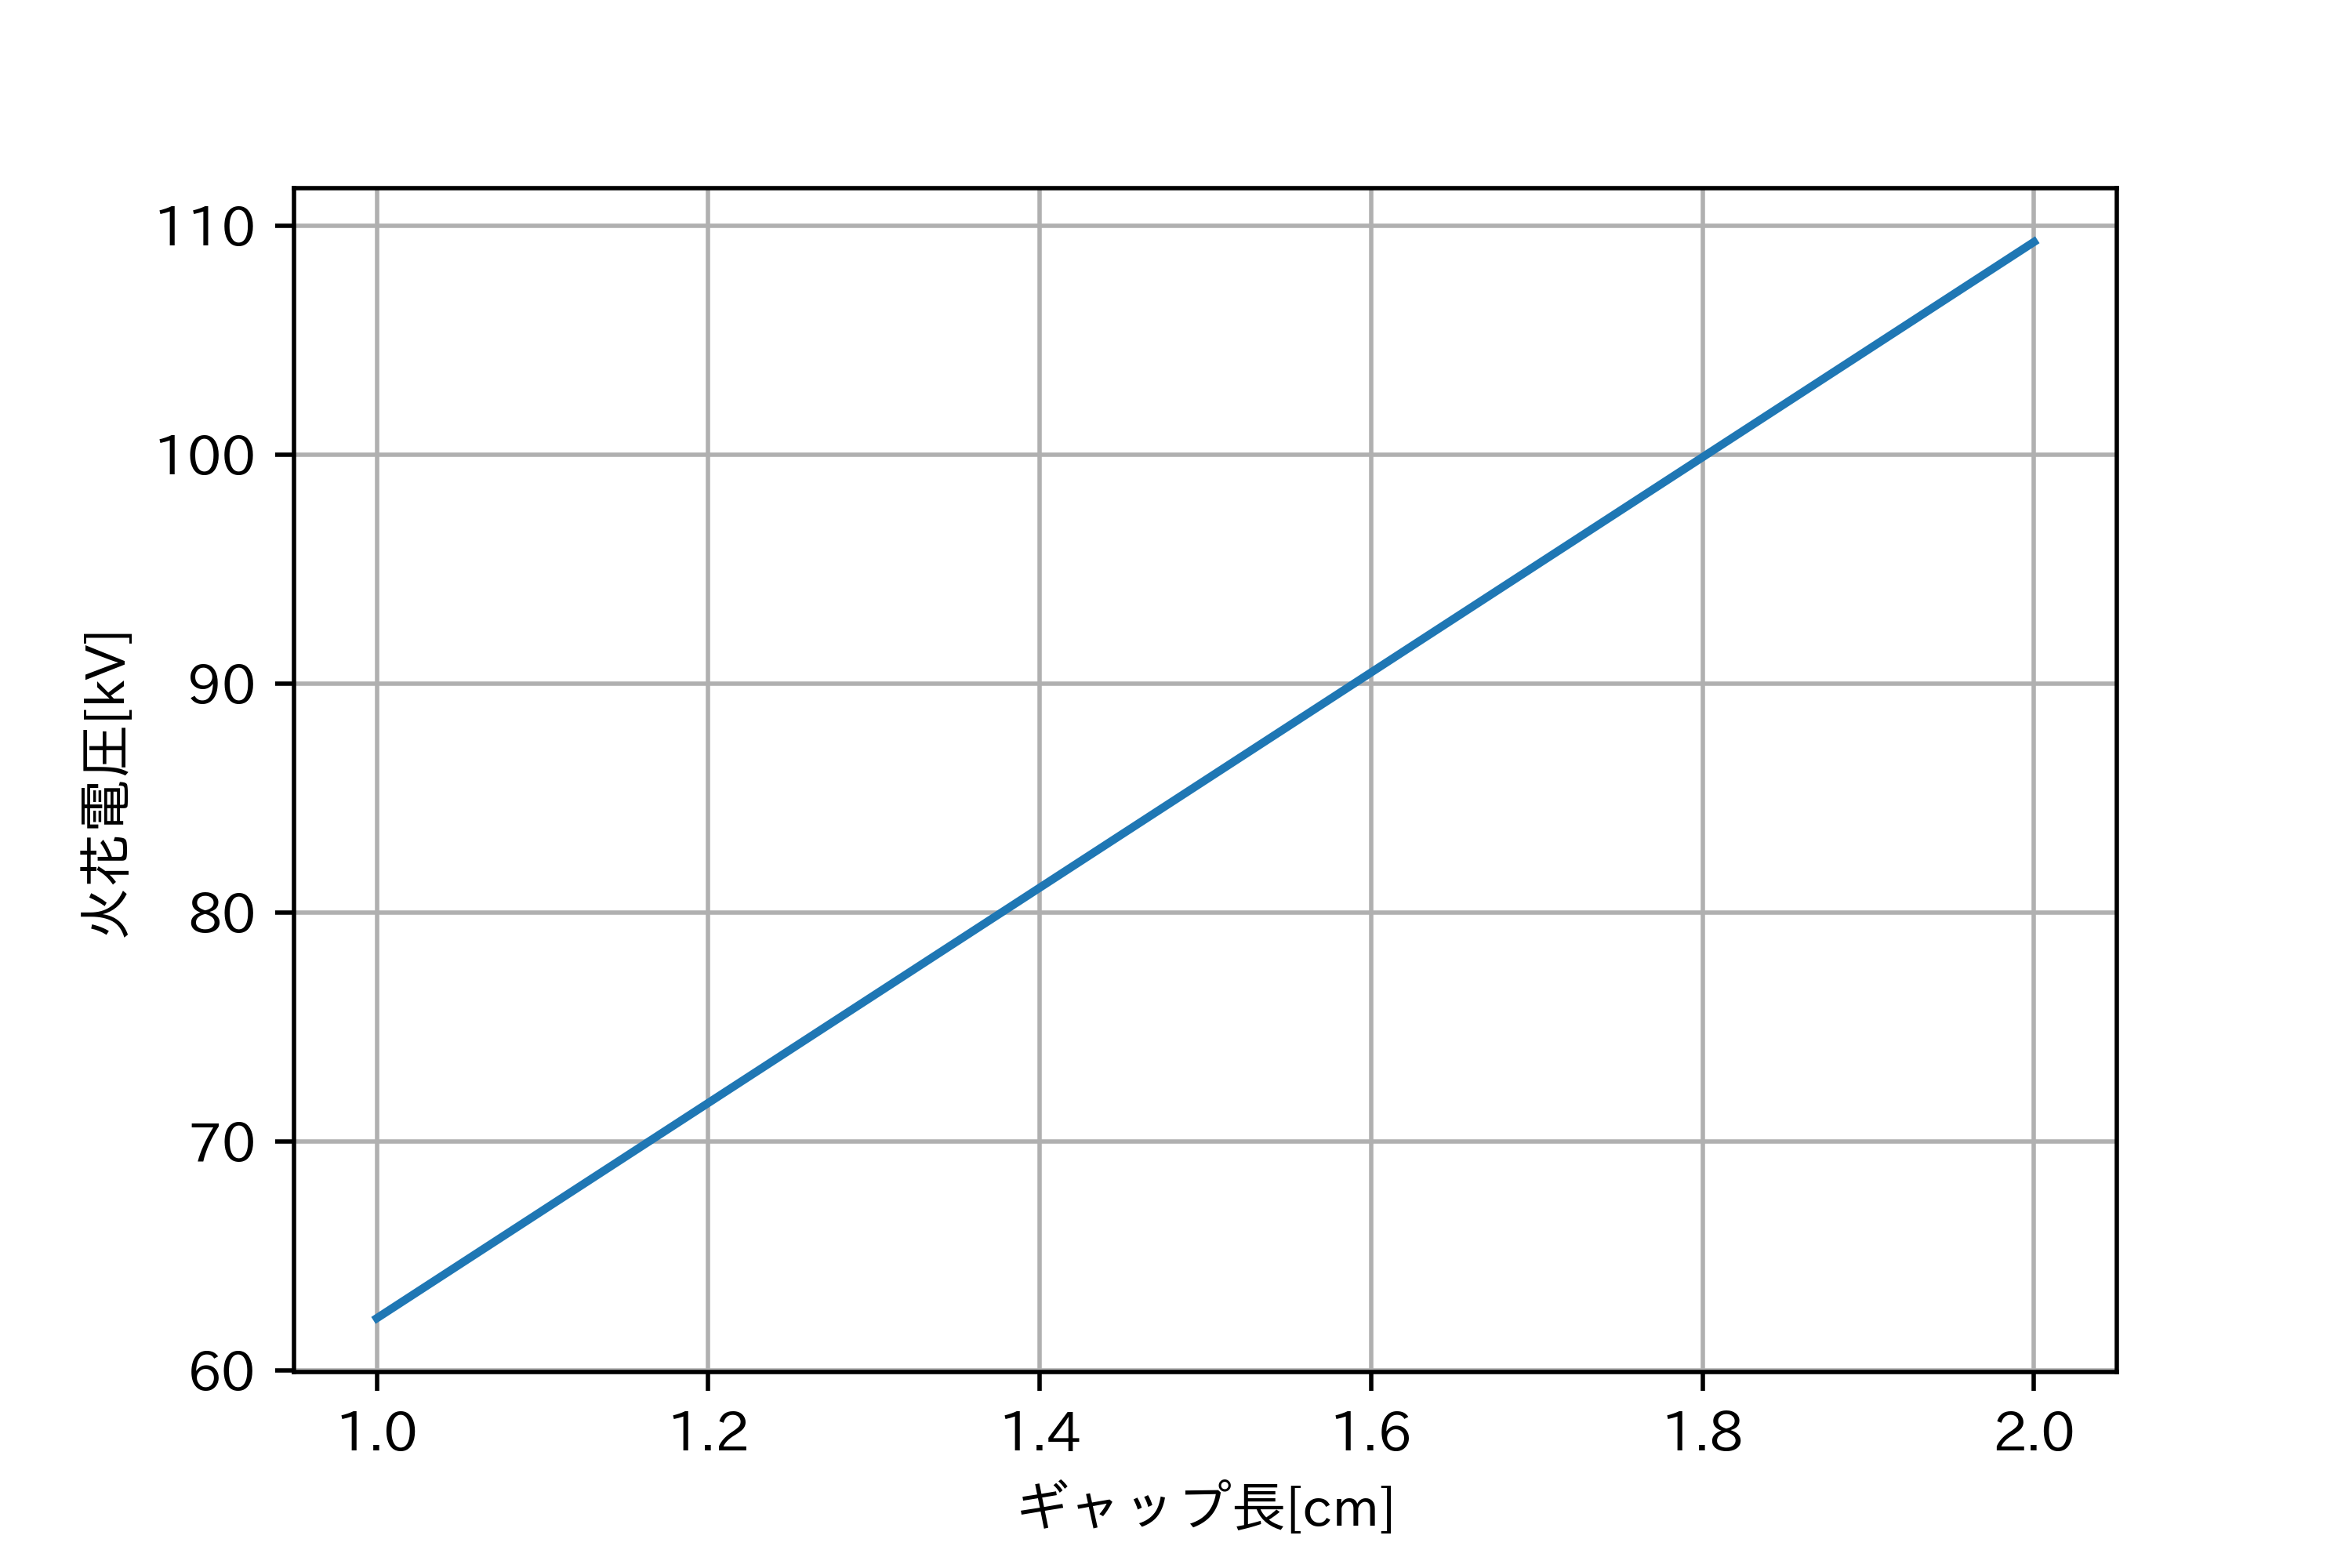
\includegraphics[scale = 0.5]{A4.png}
\caption{SF$_{6}$中の火花特性}
\end{center}
\end{figure}
大気中に比べるとかなり火花電圧が高くなっていることがわかる。
\subsubsection*{A5. がい子のフラッシュオーバ電圧}

\begin{figure}[H]
\begin{center}
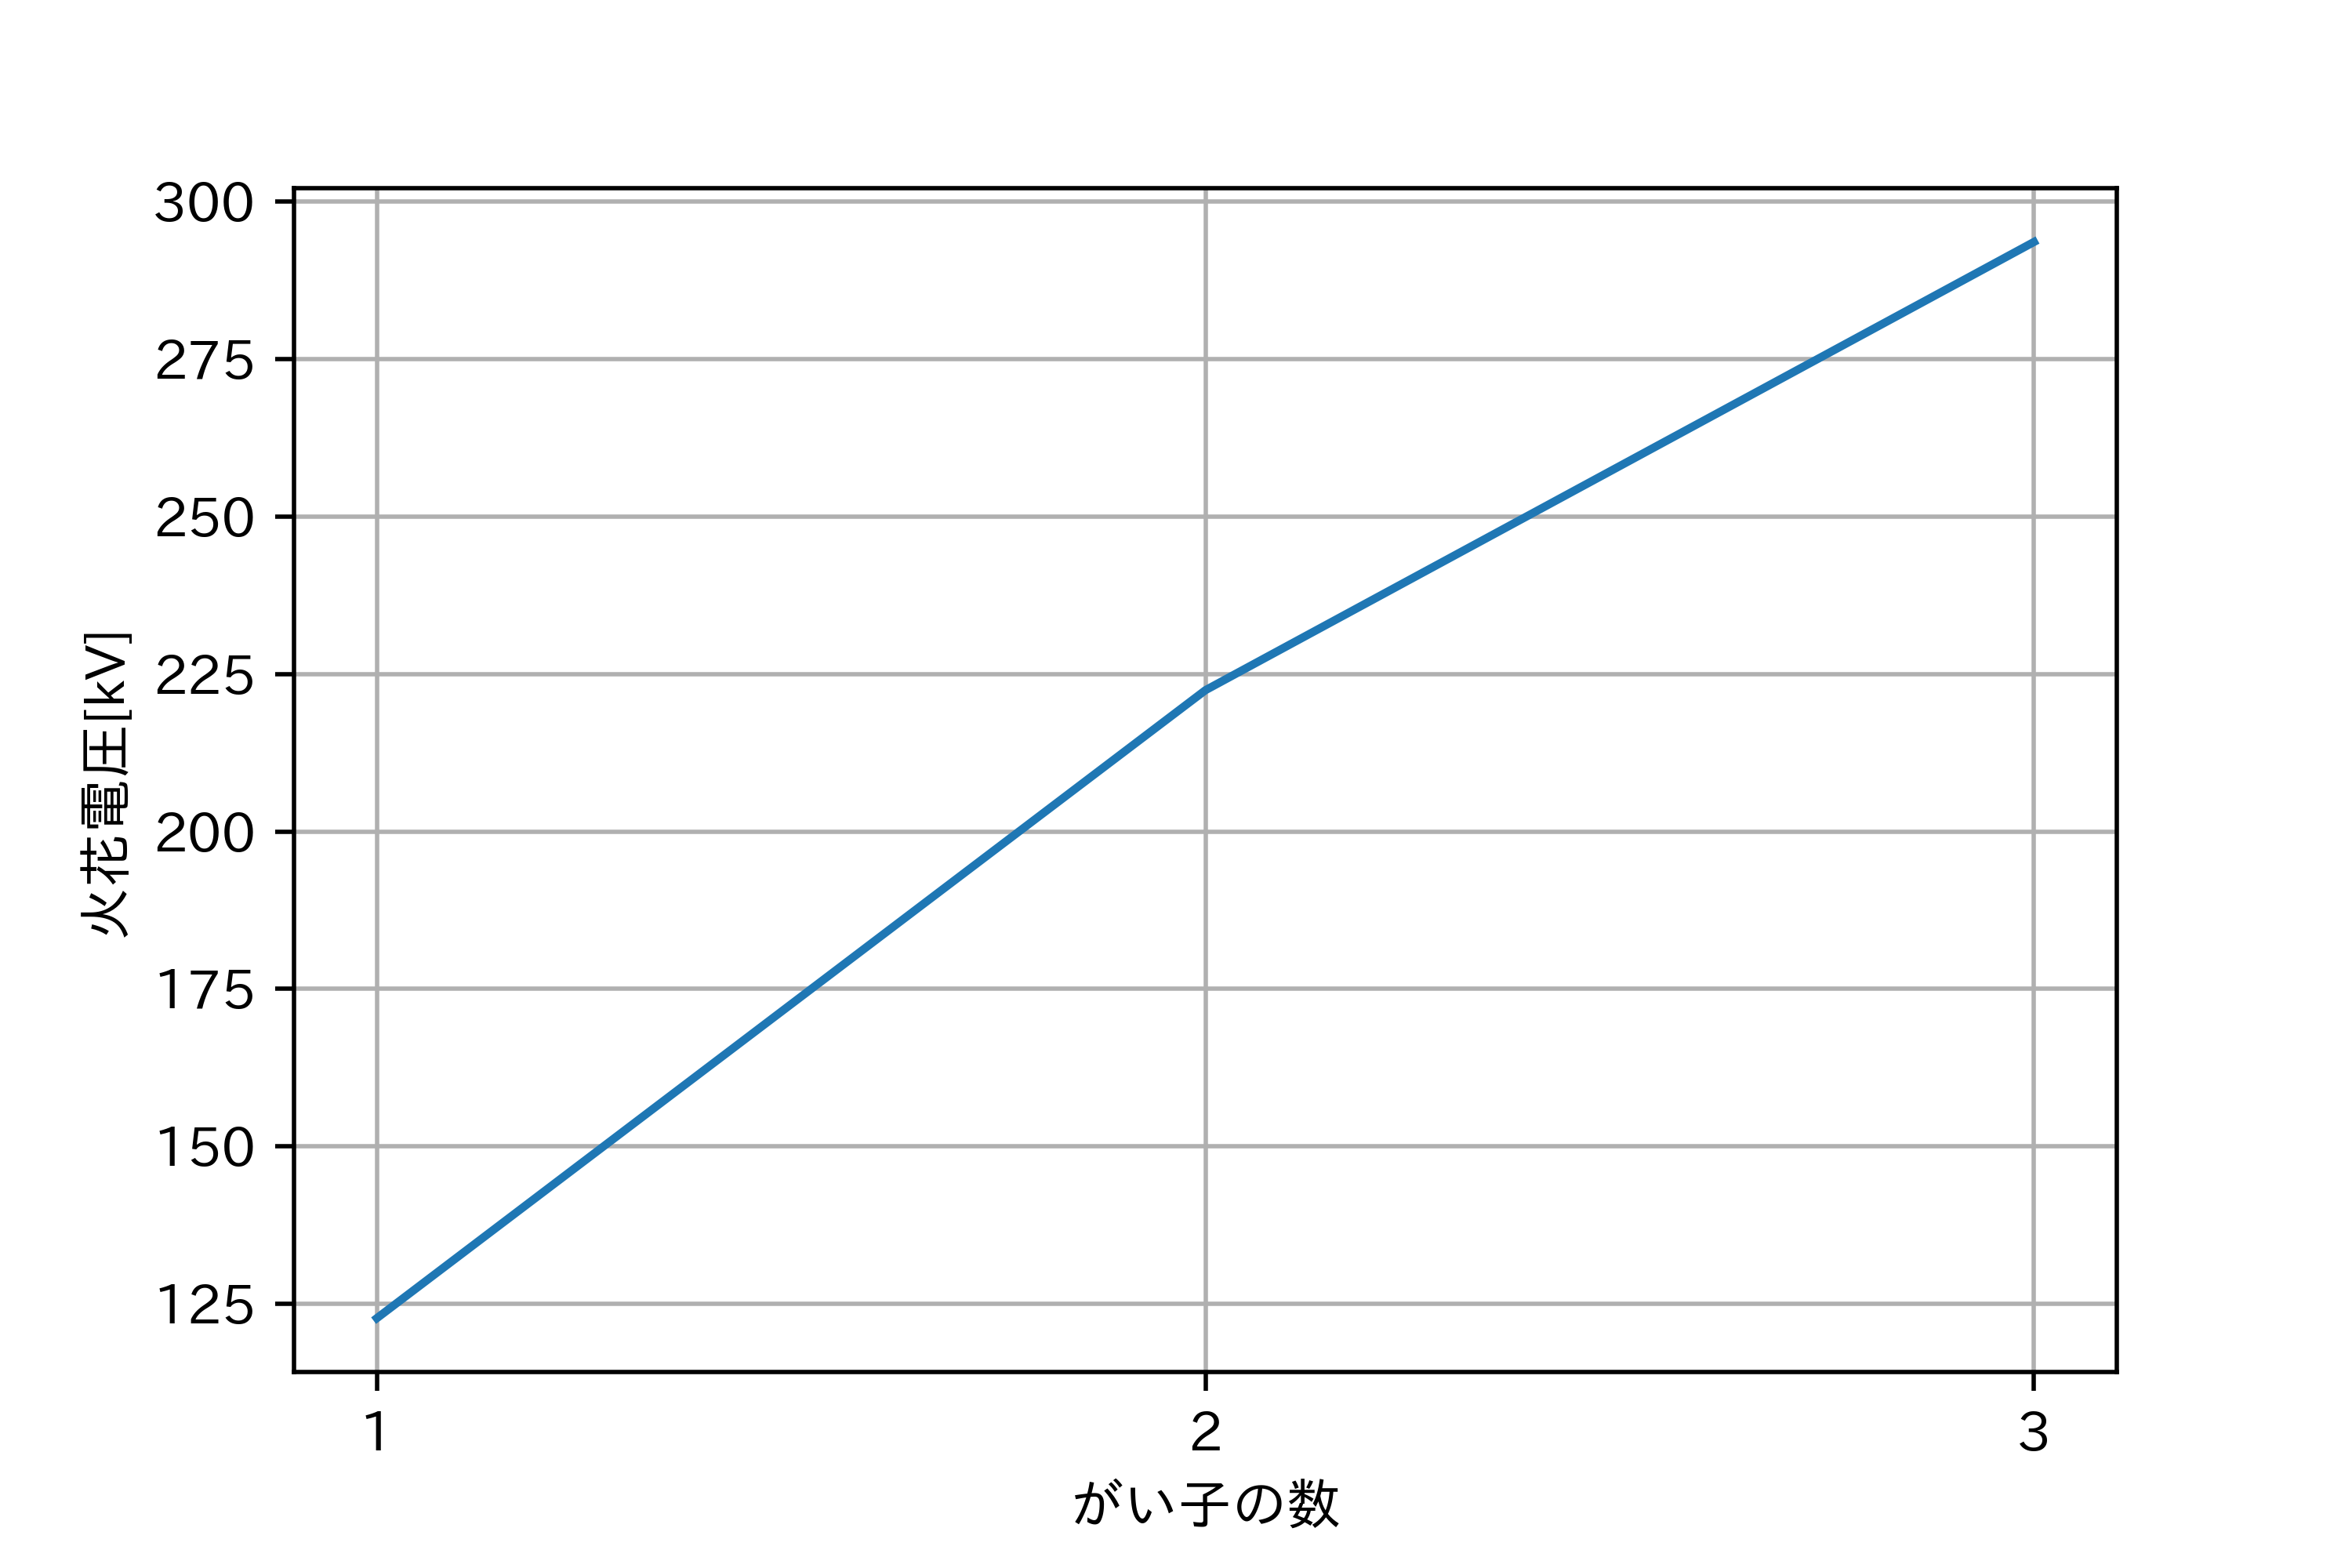
\includegraphics[scale = 0.5]{A5.png}
\caption{がい子のフラッシュオーバ電圧}
\end{center}
\end{figure}
がい子が増えるとゆるい傾きで火花電圧が上がっていくことがわかる。

\subsubsection*{A6. 沿面フラッシュオーバ電圧}

\begin{figure}[H]
\begin{center}
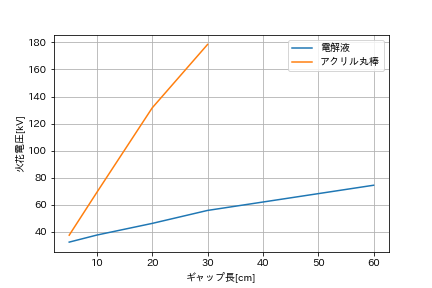
\includegraphics[scale = 0.5]{A6.png}
\caption{沿面フラッシュオーバ電圧}
\end{center}
\end{figure}
アクリルの方の火花電圧が電解液の火花電圧よりかなり高くなっていることがわかる。

\subsection*{B. 直流高電圧}

\subsubsection*{B1. 針-平板ギャップの火花特性}
\begin{figure}[H]
\begin{center}
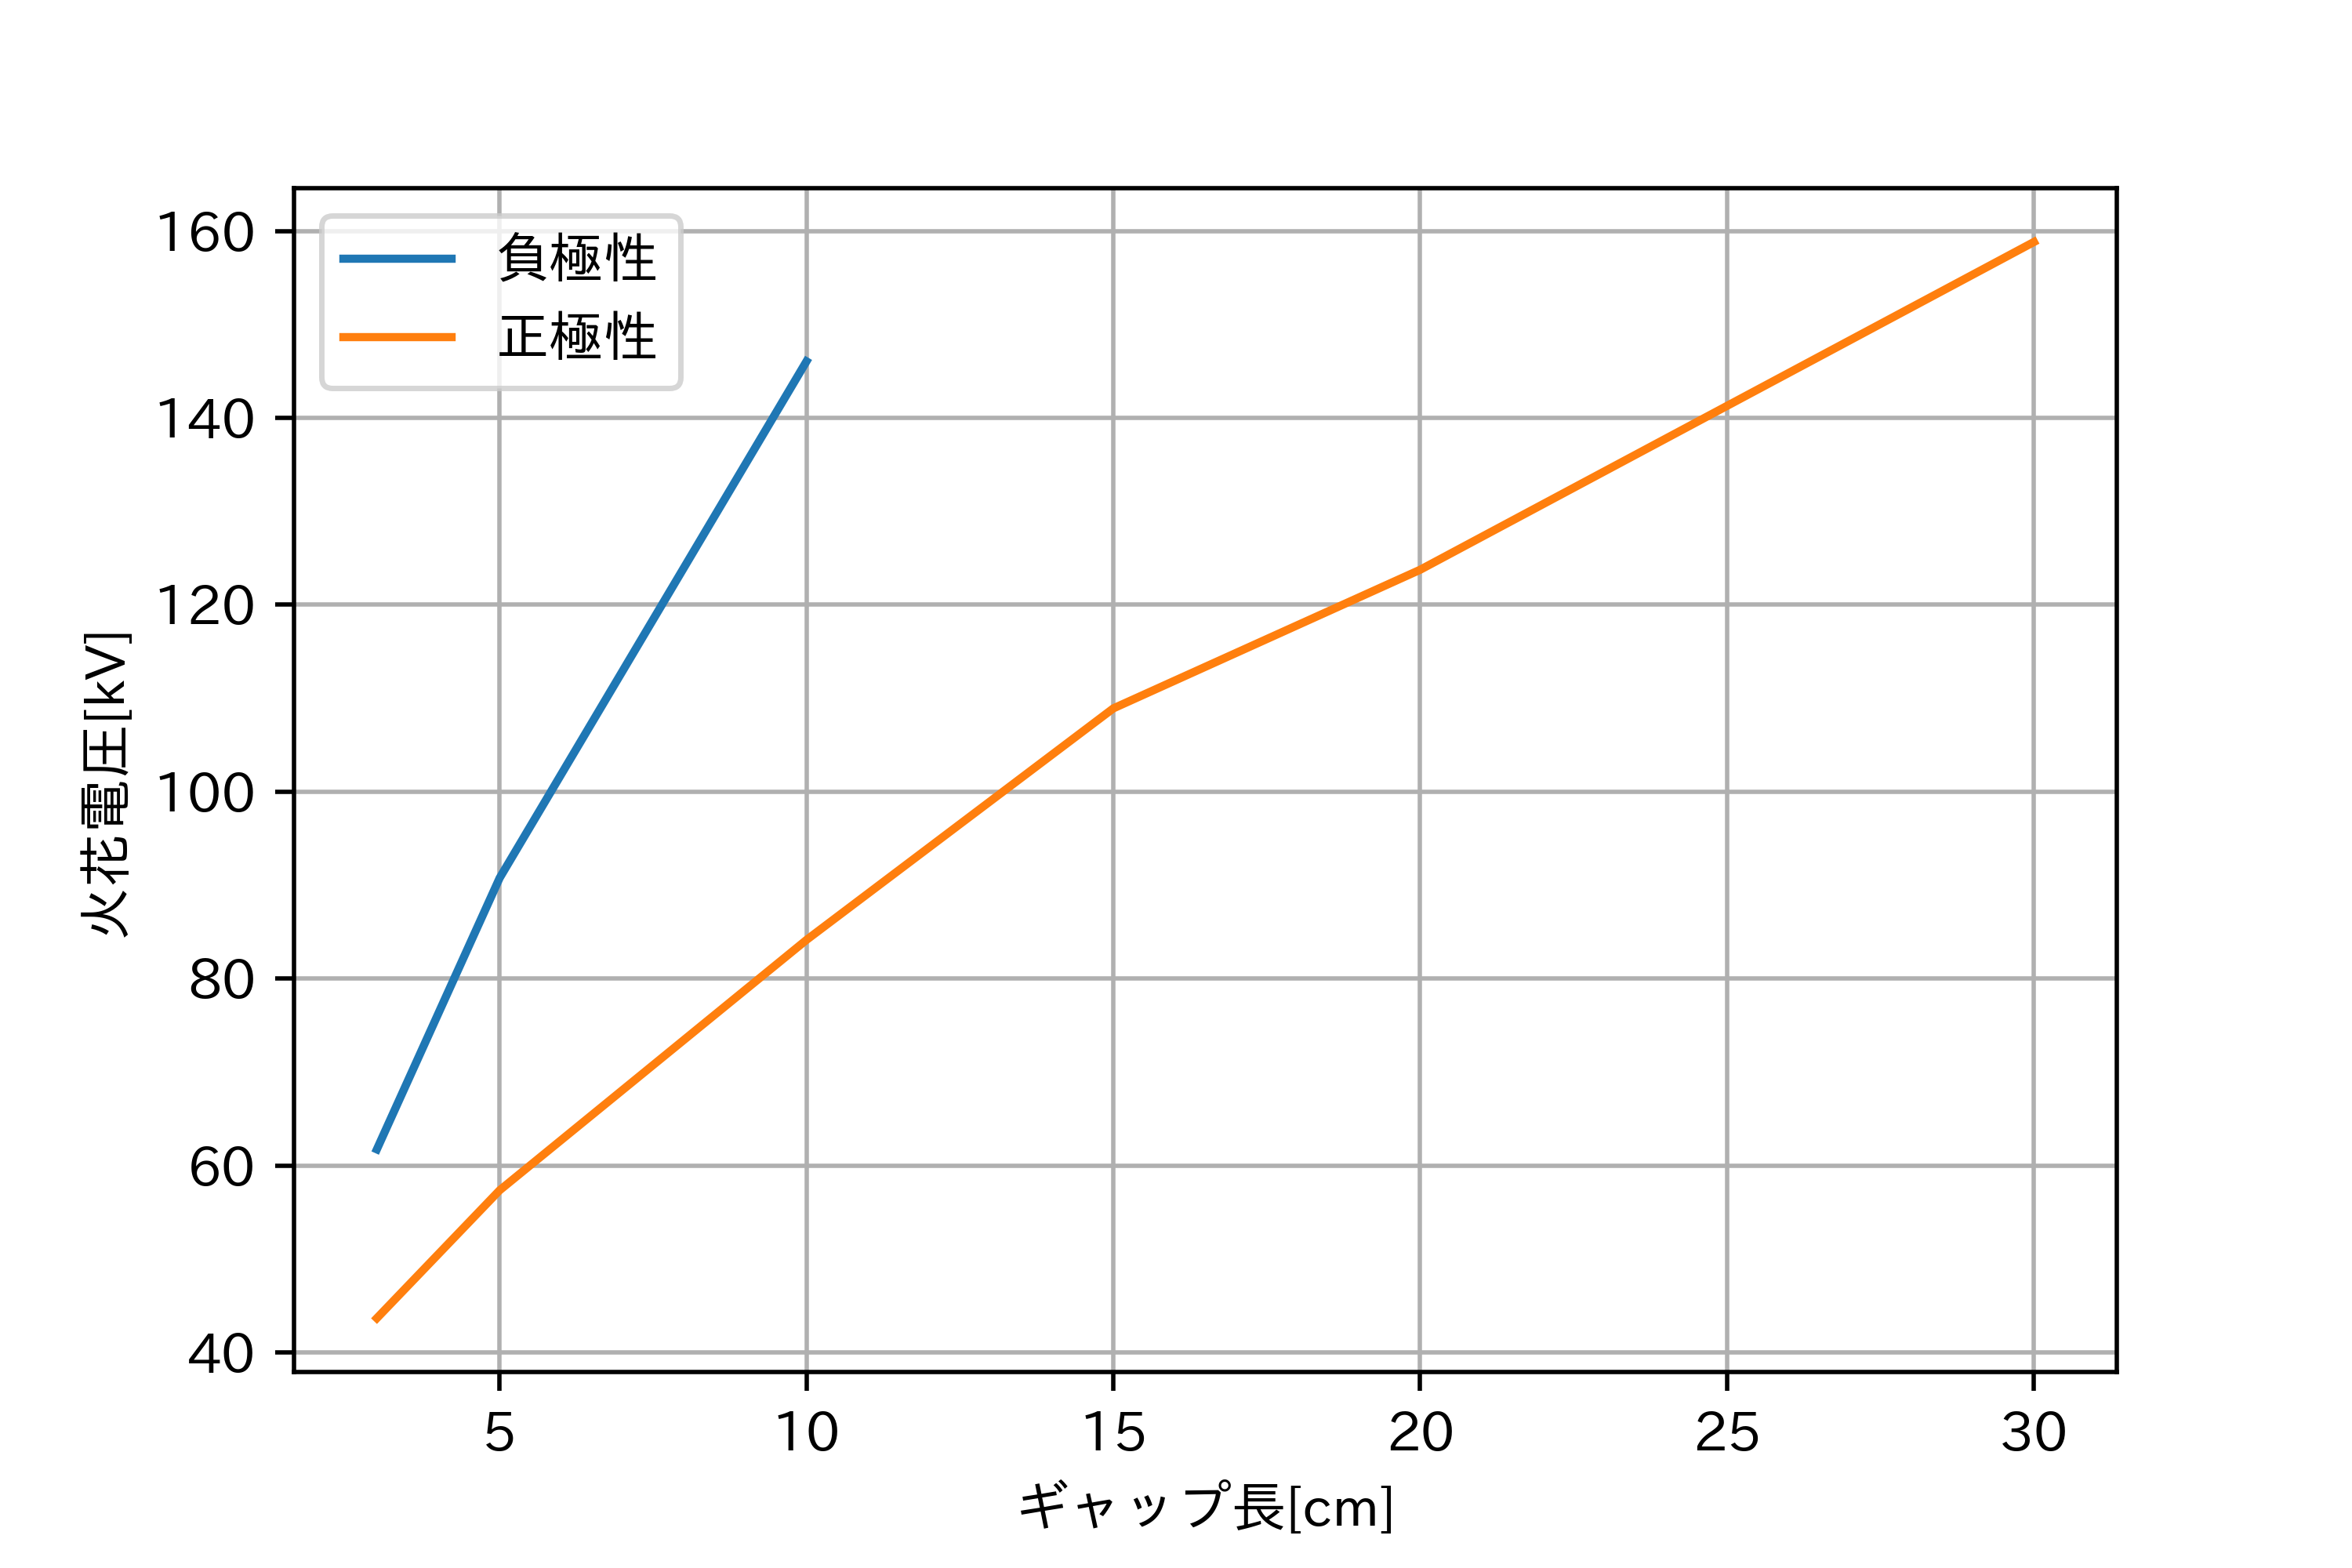
\includegraphics[scale = 0.5]{B1.png}
\caption{針-平板ギャップの火花特性}
\end{center}
\end{figure}

極性効果が現れ、針が接地されている時の火花電圧が高くなっていることがわかる。
\subsubsection*{B2. 棒-棒ギャップの火花特性}
負極性で記録した。
\begin{figure}[H]
\begin{center}
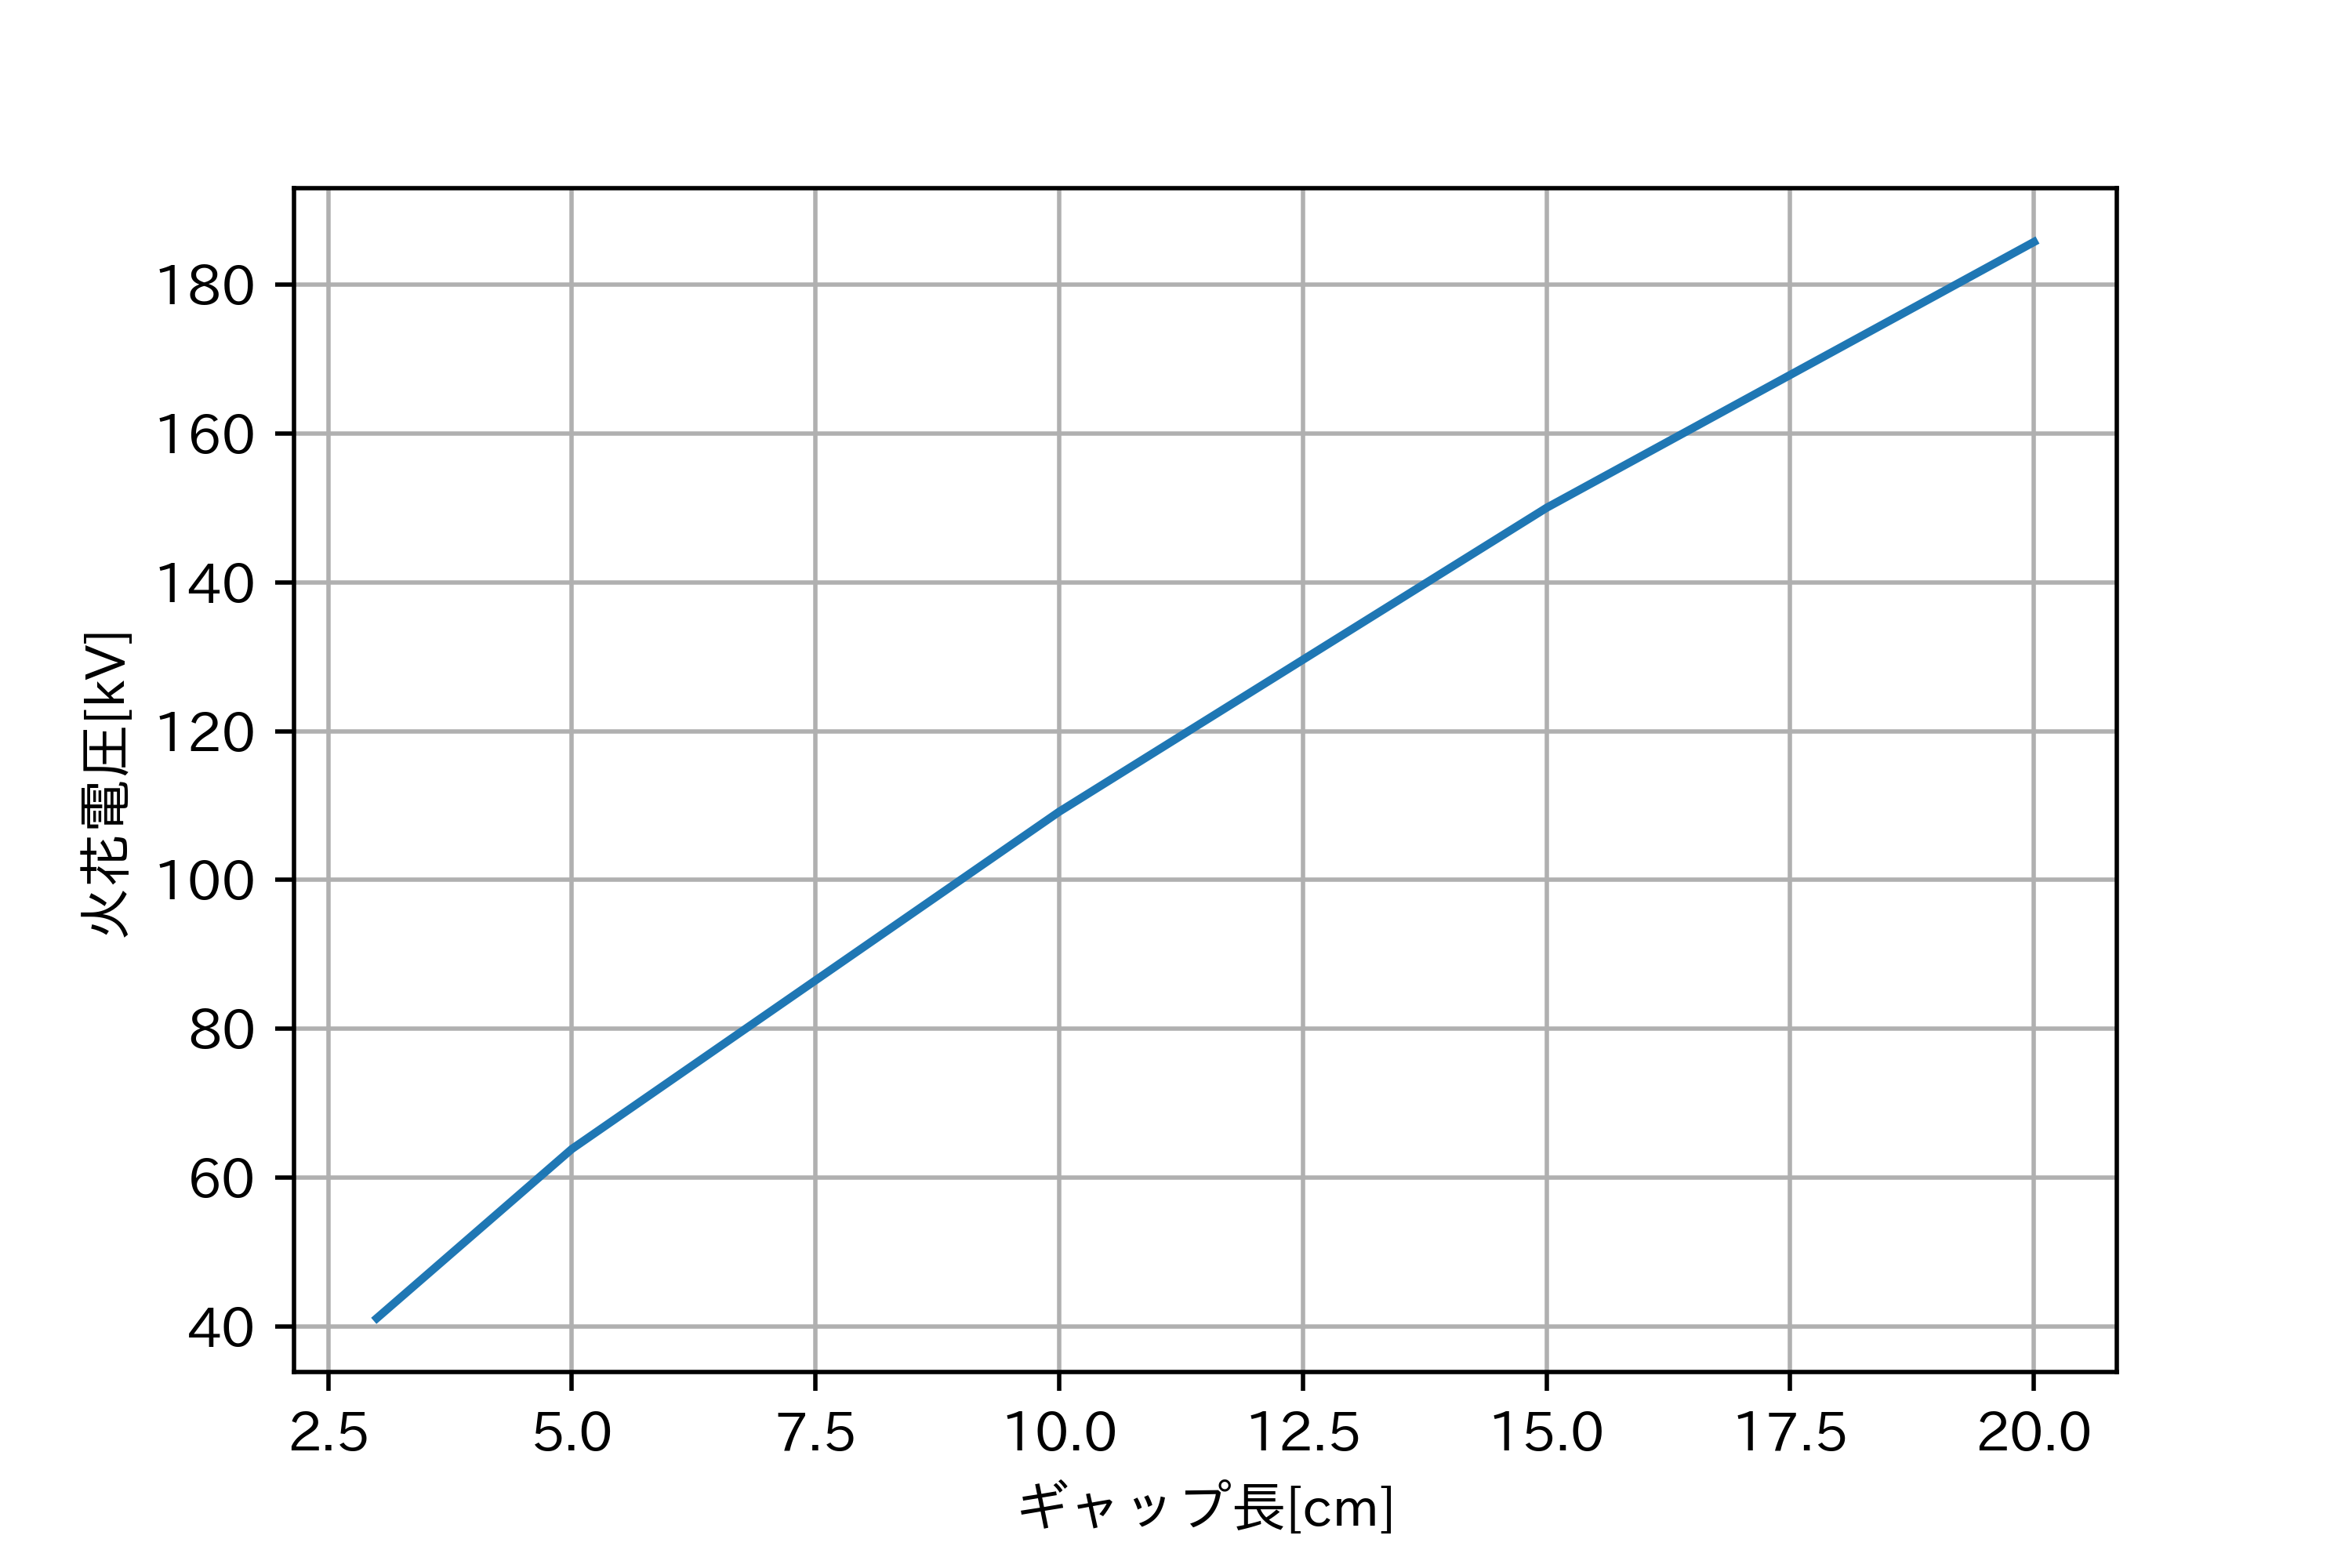
\includegraphics[scale = 0.5]{B2.png}
\caption{針-平板ギャップの火花特性}
\end{center}
\end{figure}
\subsection*{C. インパルス高電圧}

\subsubsection*{C1. インパルス高電圧発生器の原理および操作法}
略
\subsubsection*{C2. 球ギャップによる電圧測定}
\begin{figure}[H]
\begin{center}
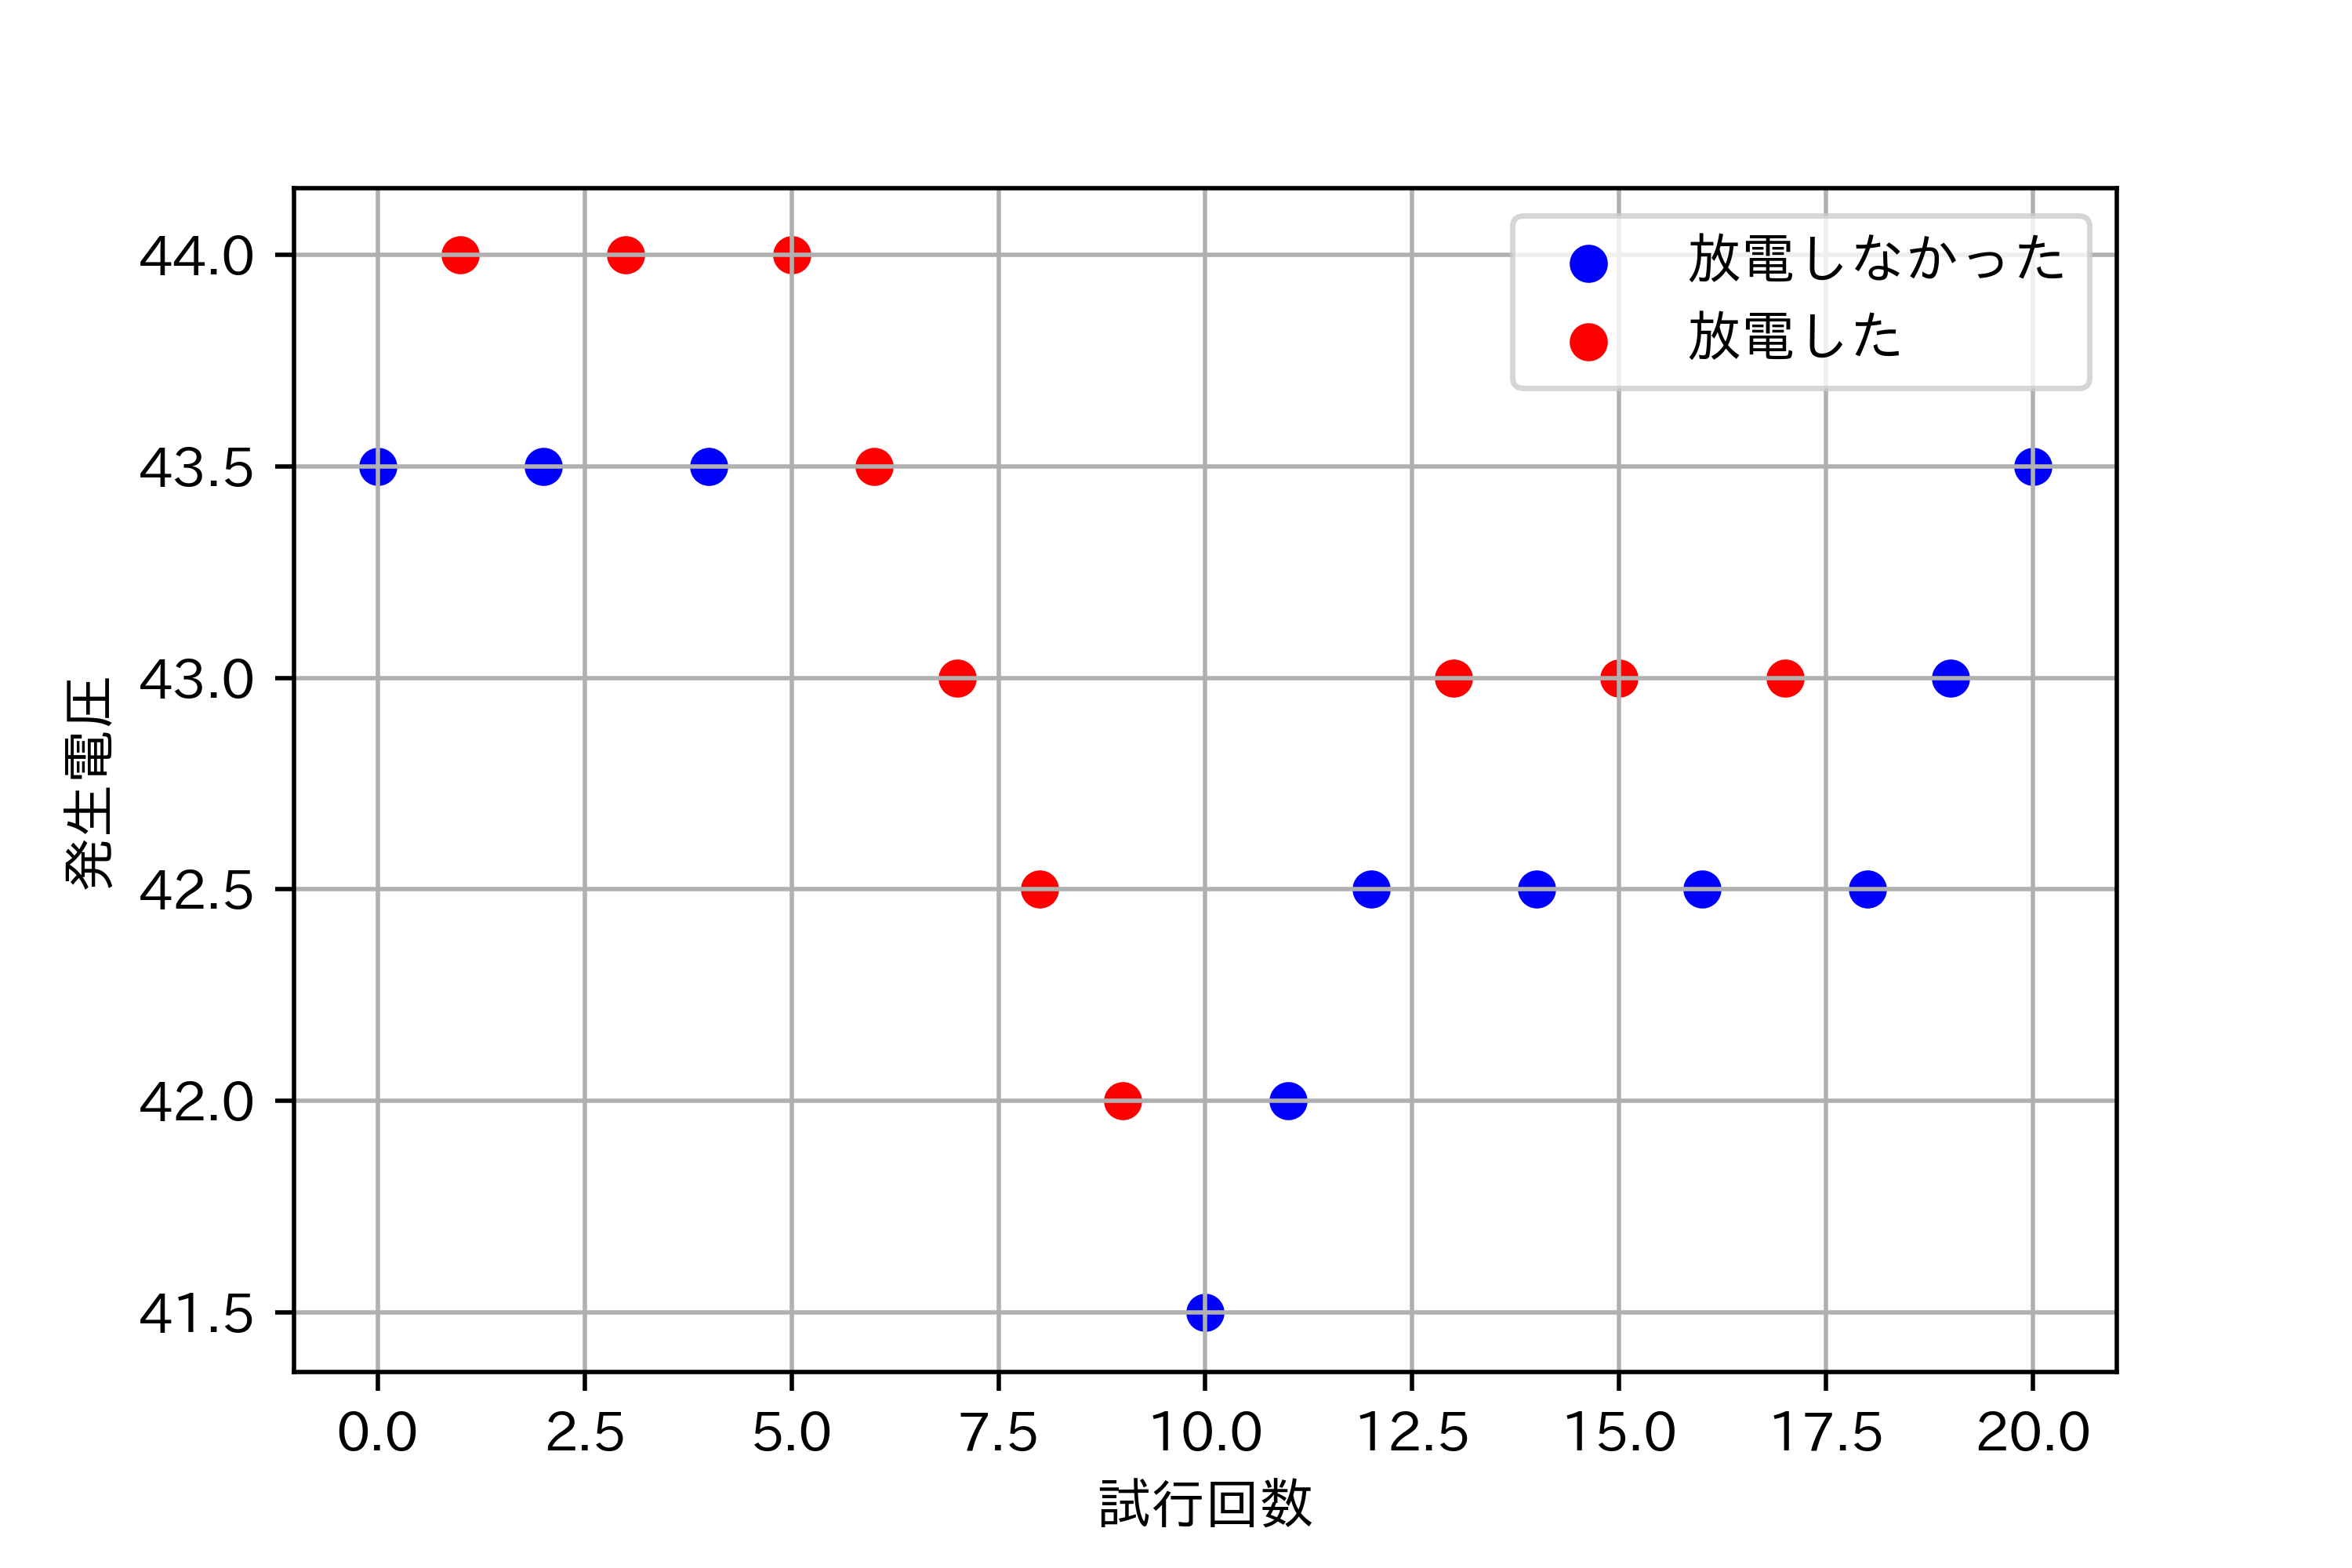
\includegraphics[scale = 0.5]{C21.png}
\caption{昇降法による測定(ギャップ長=90mm)}
\end{center}
\end{figure}

\begin{figure}[H]
\begin{center}
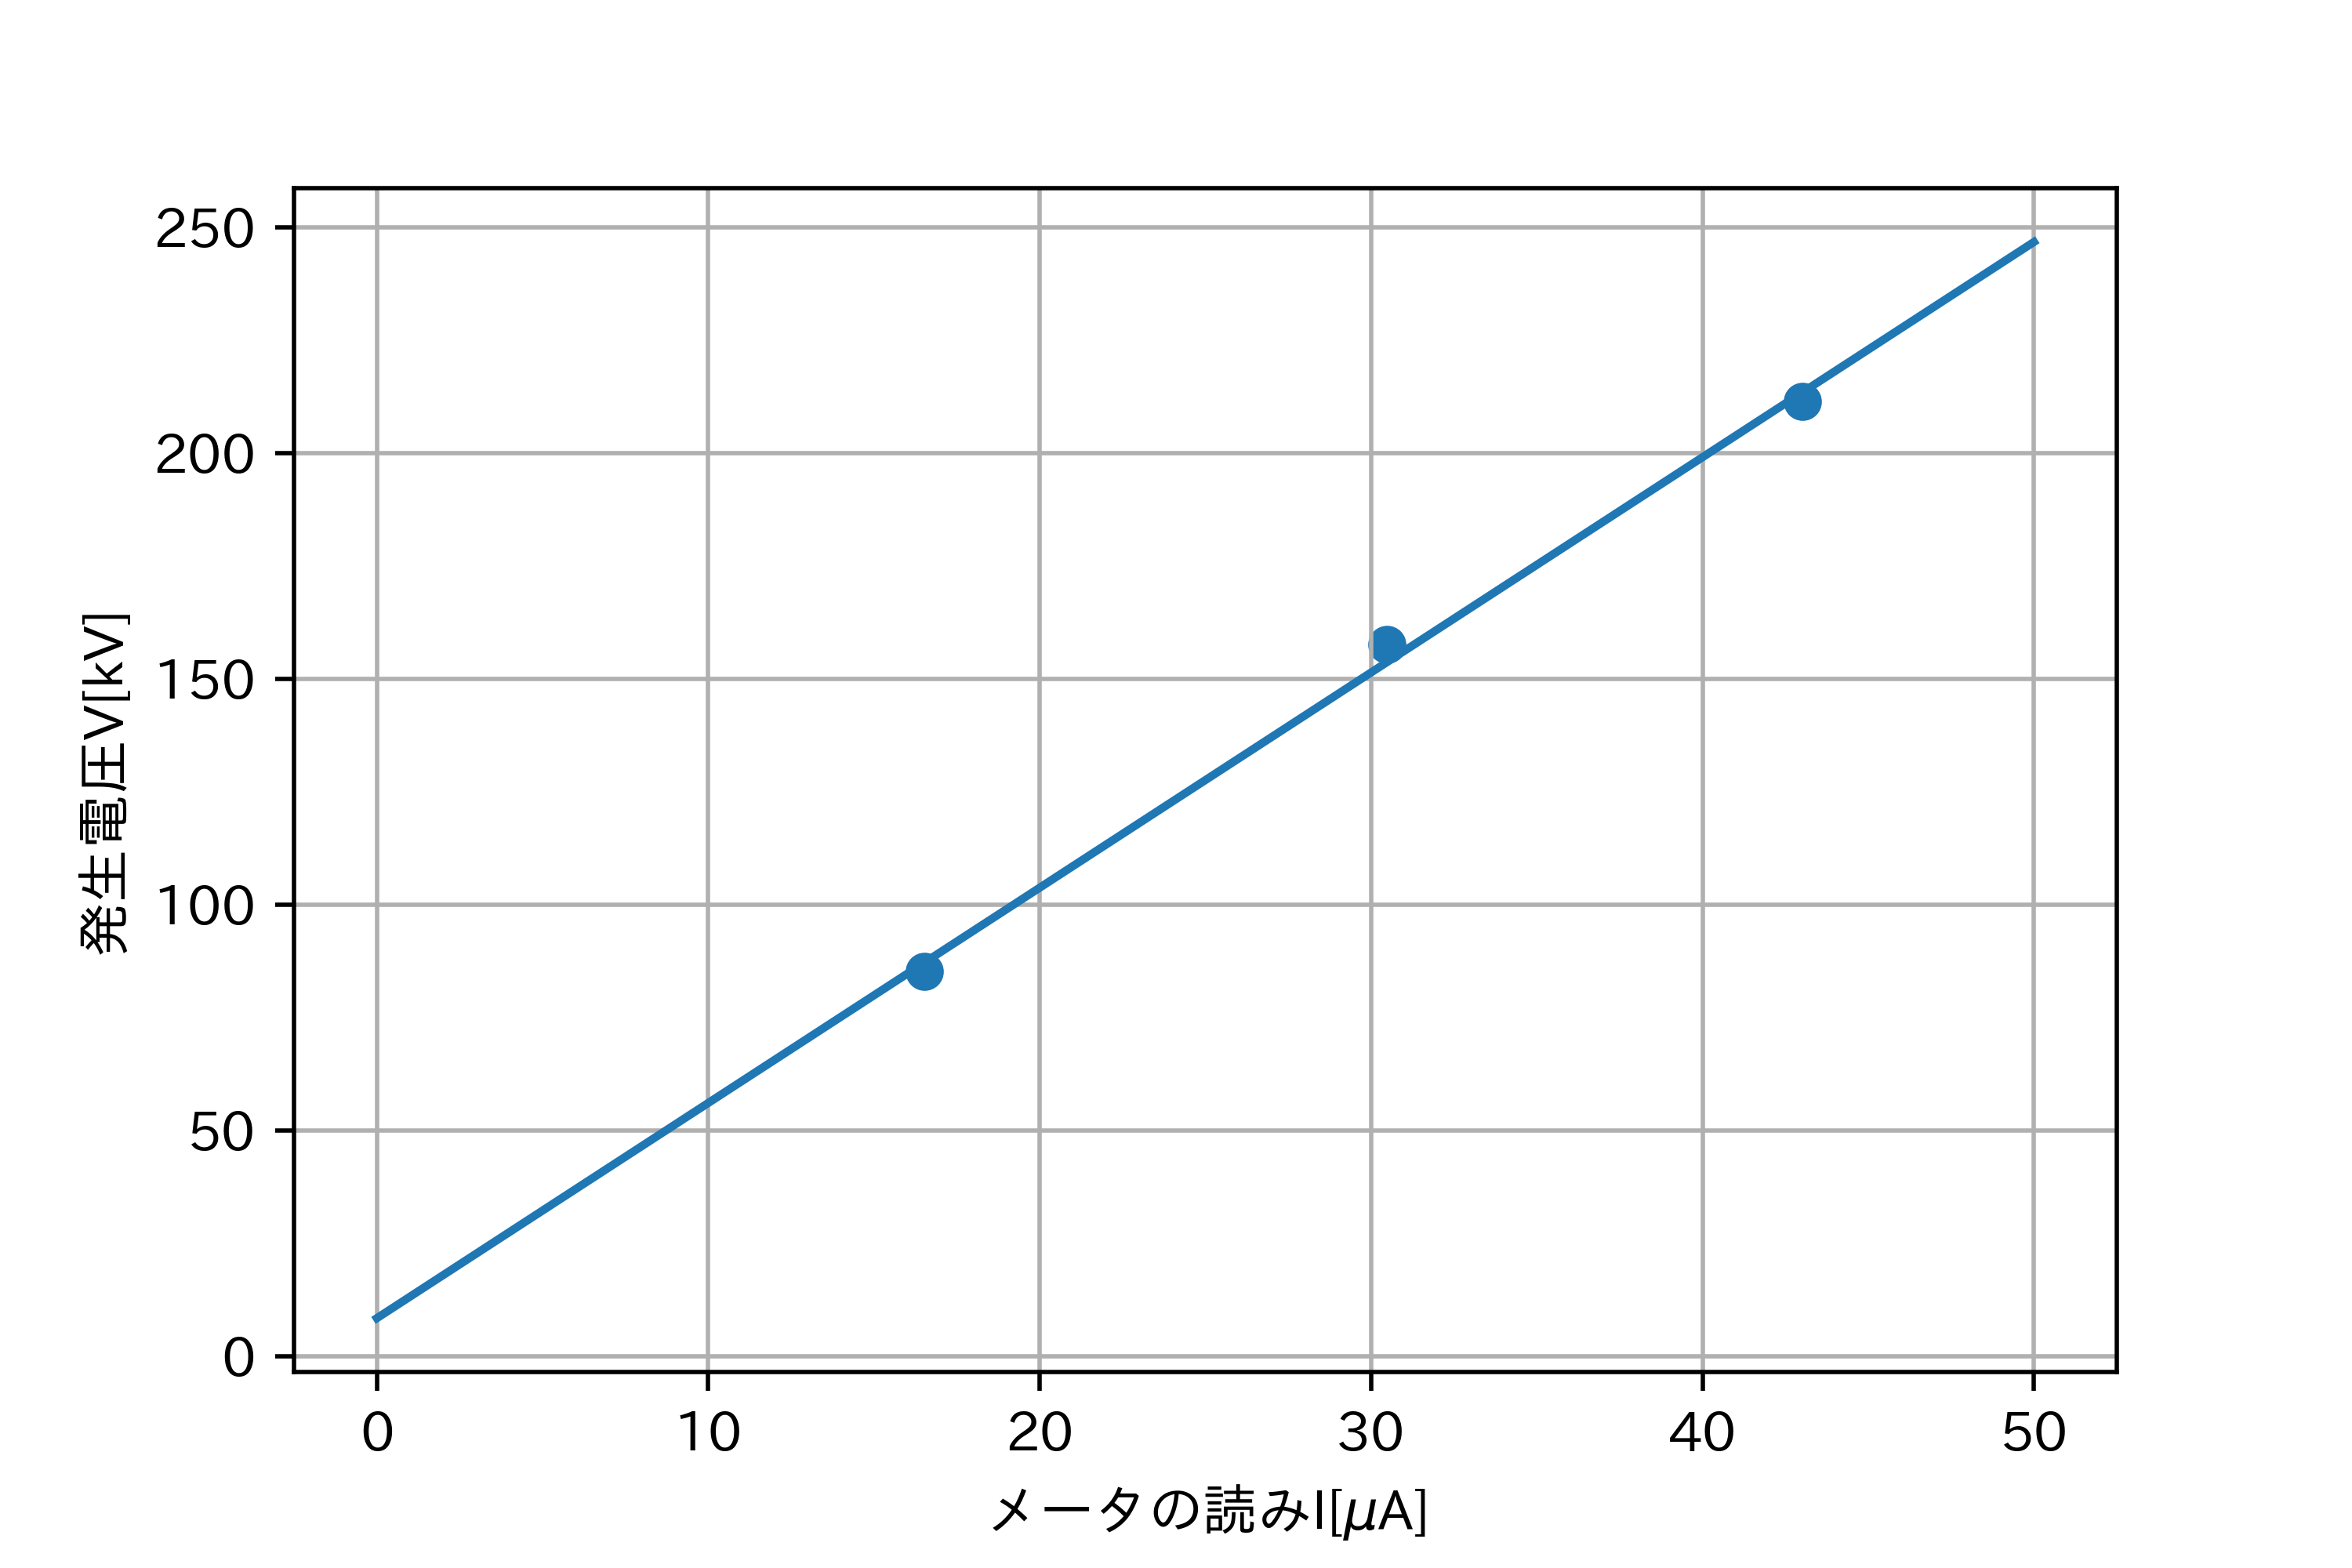
\includegraphics[scale = 0.5]{C22.png}
\caption{発生電圧の校正曲線}
\end{center}
\end{figure}

発生電圧$V$は電流計の読み$I$に対して

$V = 4.7\times I +8.3$と校正された。

\begin{figure}[H]
\begin{center}
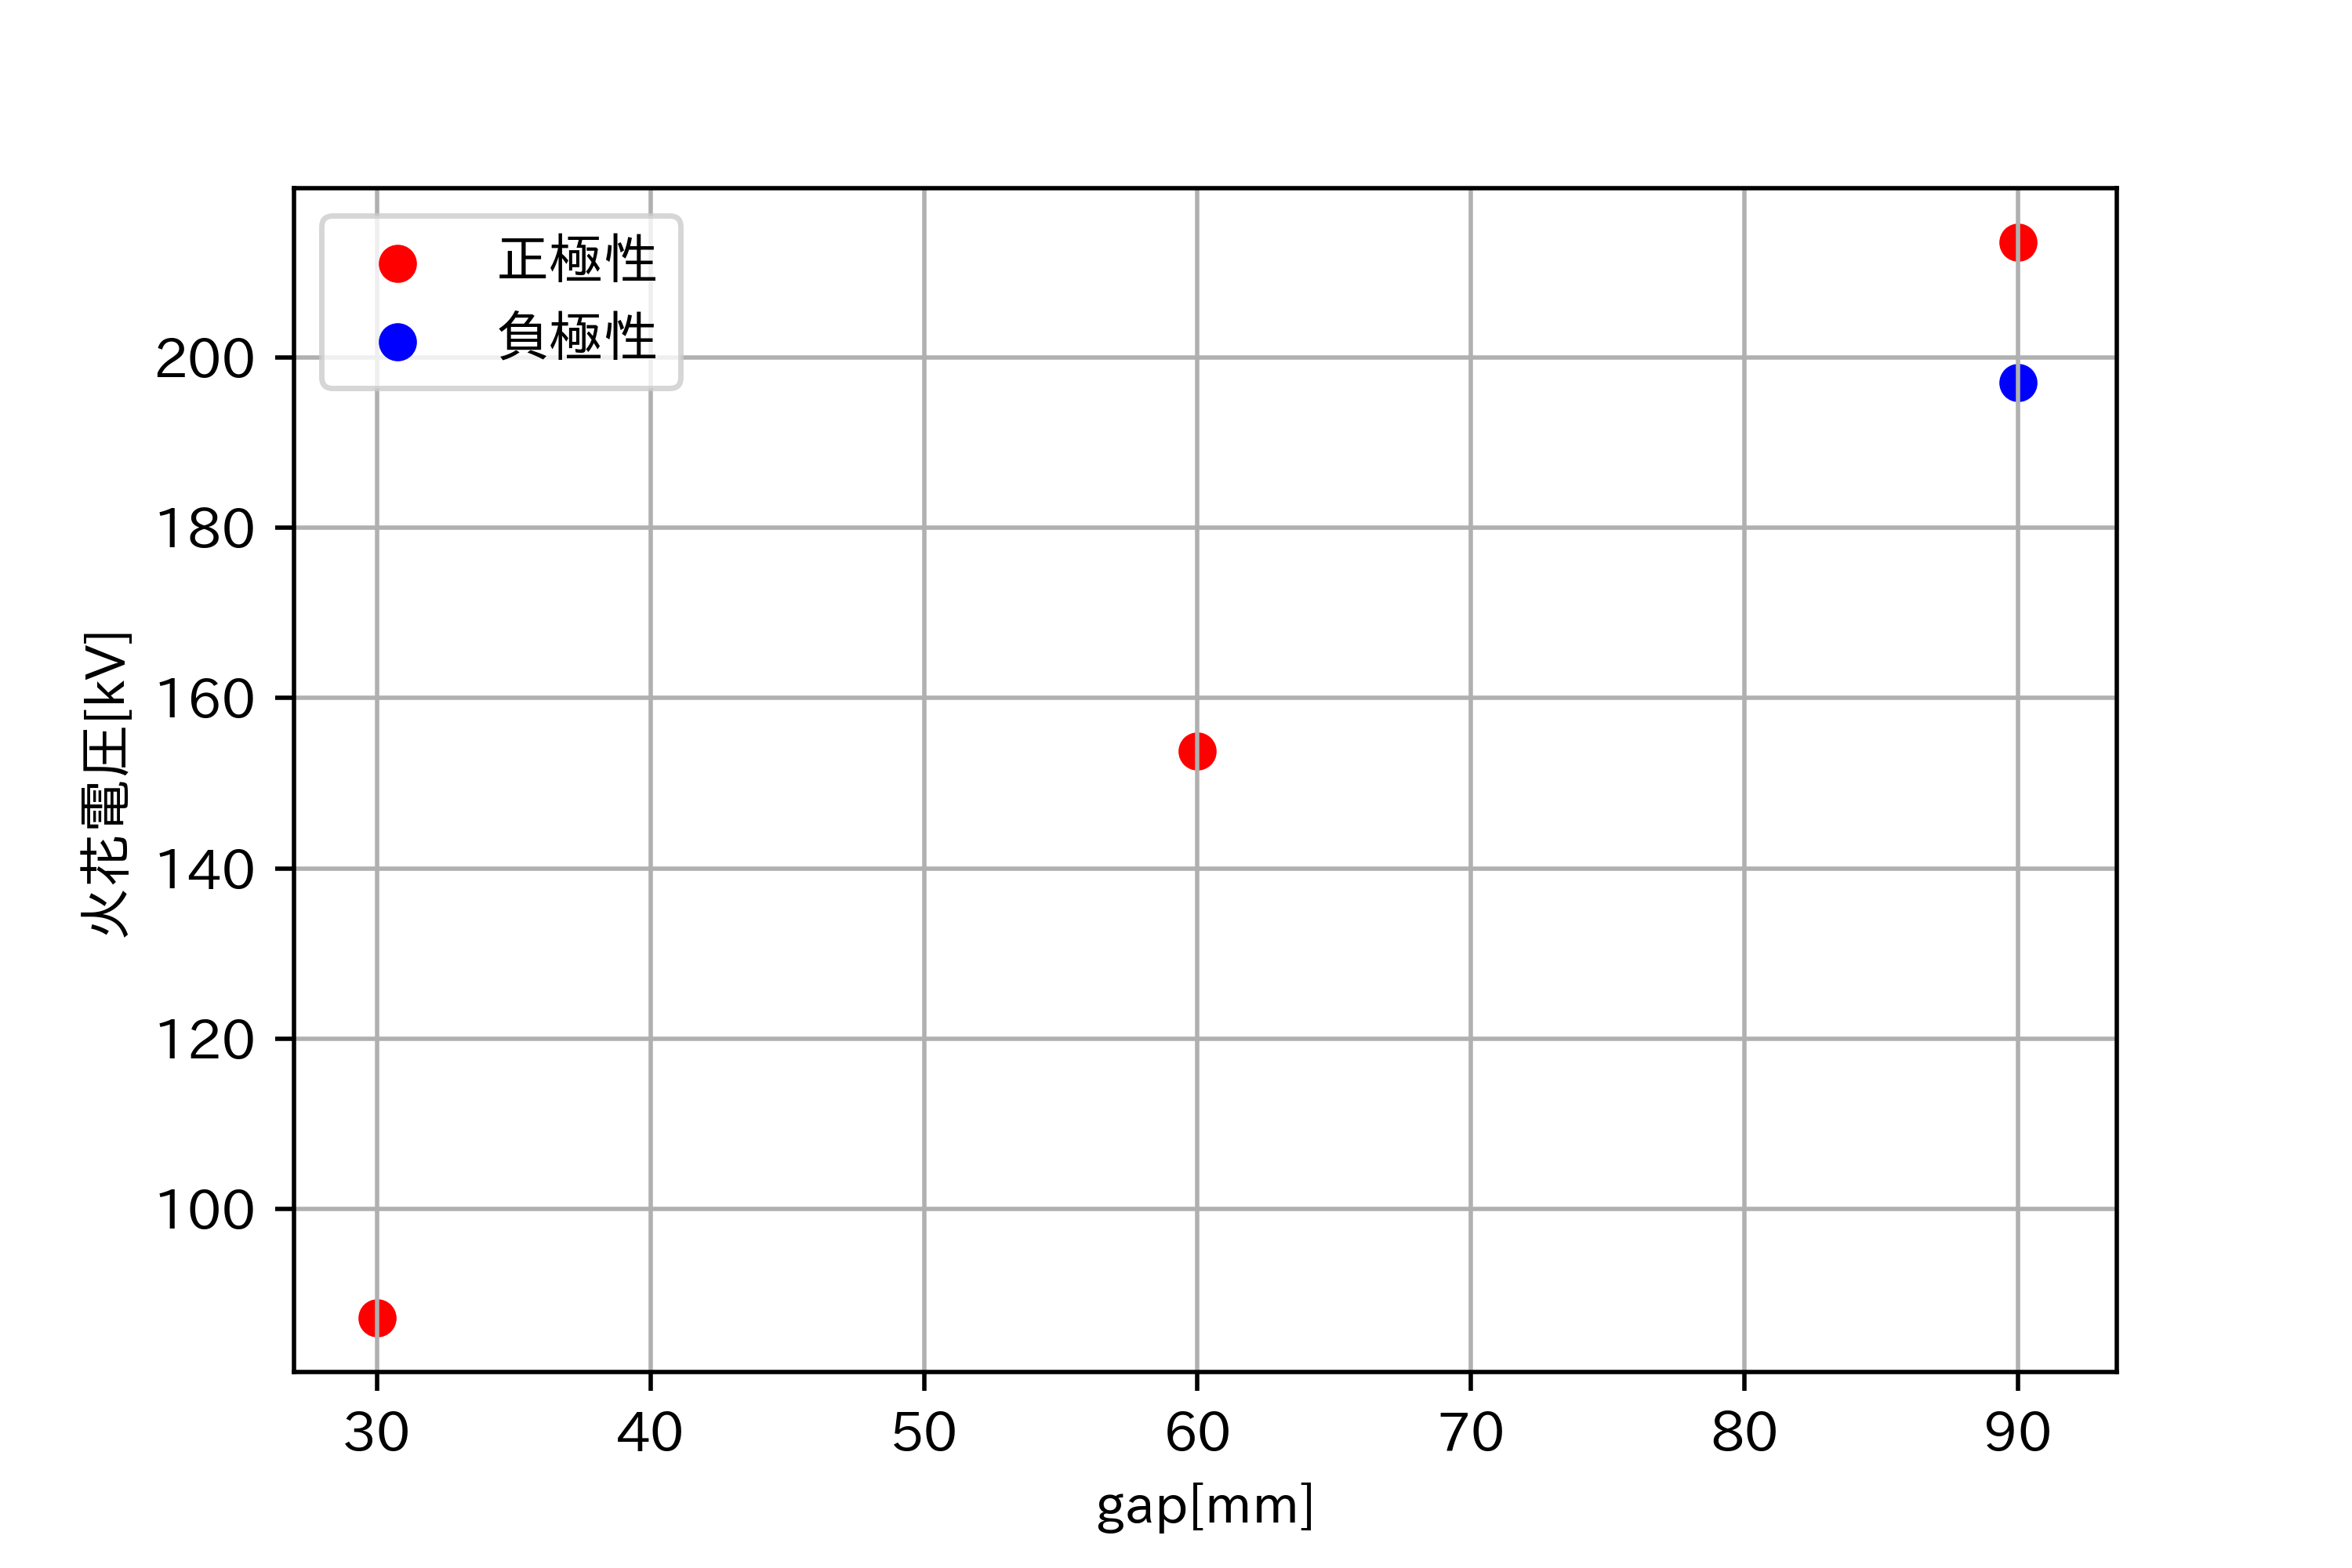
\includegraphics[scale = 0.5]{C2.png}
\caption{インパルス高電圧(球ギャップ)の極性効果}
\end{center}
\end{figure}
負極性の火花電圧がやや低い。
\subsubsection*{C3. がい子のフラッシュオーバ電圧}
\begin{figure}[H]
\begin{center}
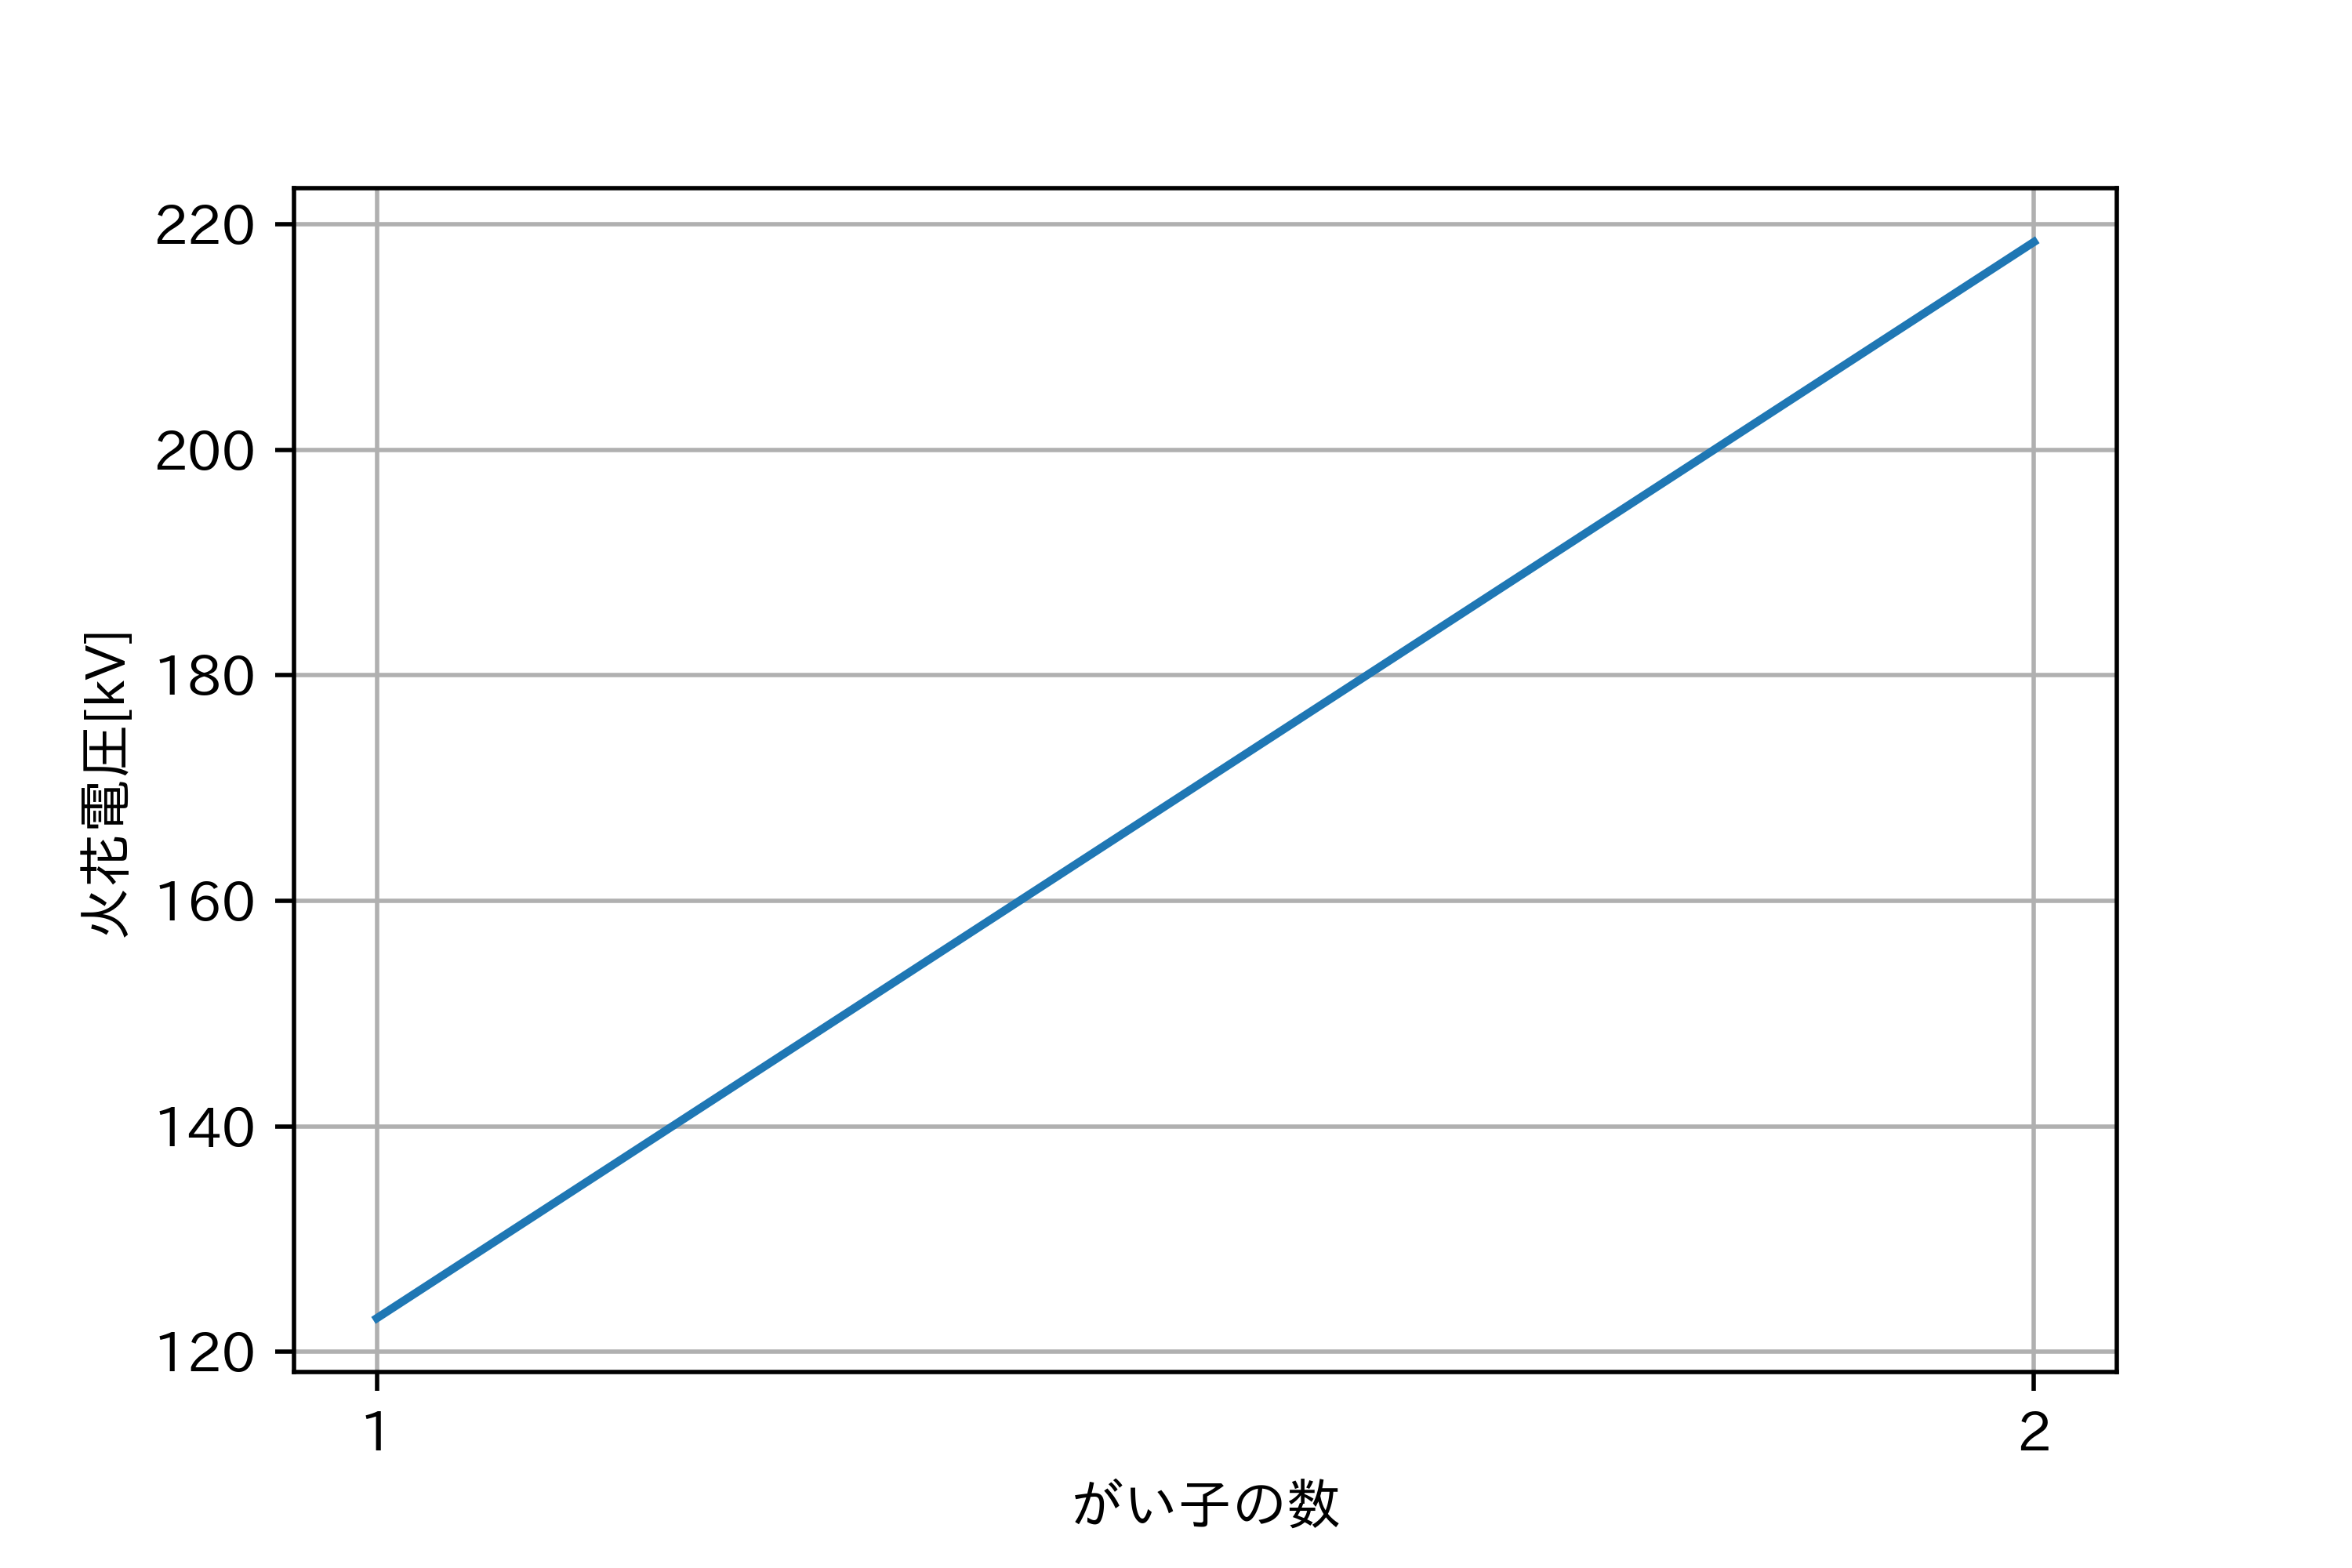
\includegraphics[scale = 0.5]{C3.png}
\caption{がい子のフラッシュオーバ電圧}
\end{center}
\end{figure}

\subsubsection*{C4. 不平等電界の火花放電率曲線}
\begin{figure}[H]
\begin{center}
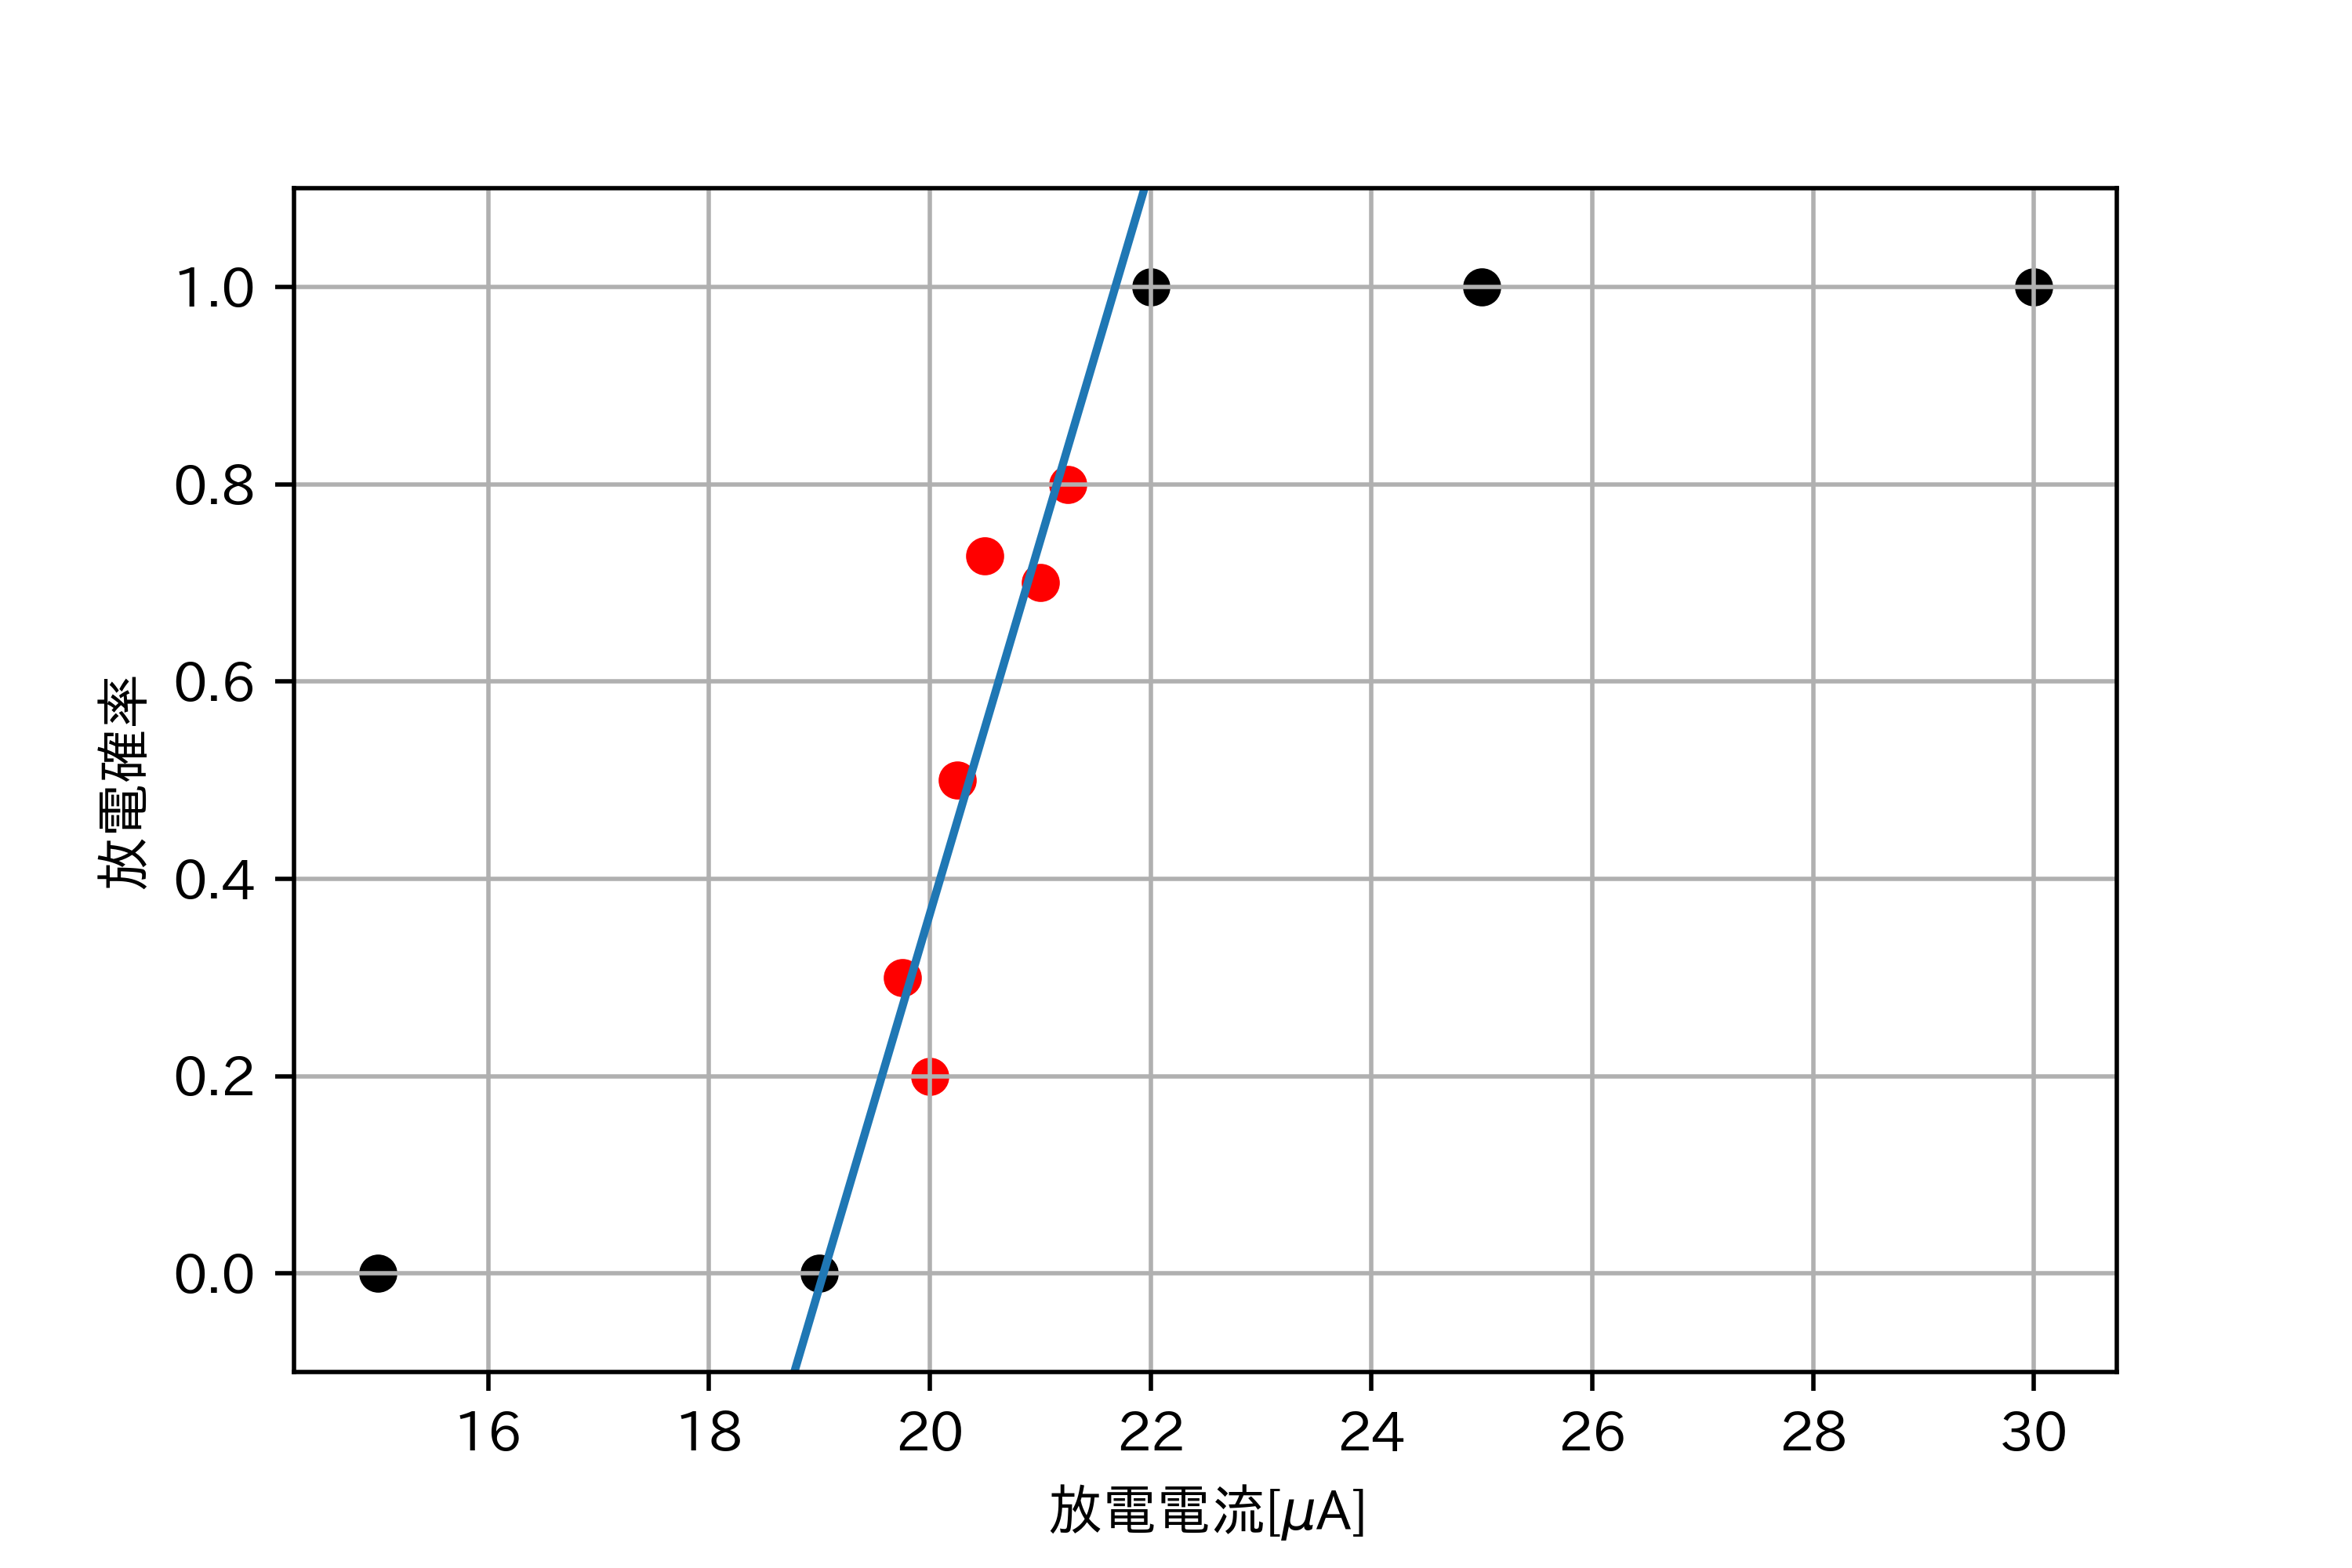
\includegraphics[scale = 0.5]{C41.png}
\caption{補間法による正極性の50\%火花電圧測定}
\end{center}
\end{figure}
50\% 電圧は29kV
\begin{figure}[H]
\begin{center}
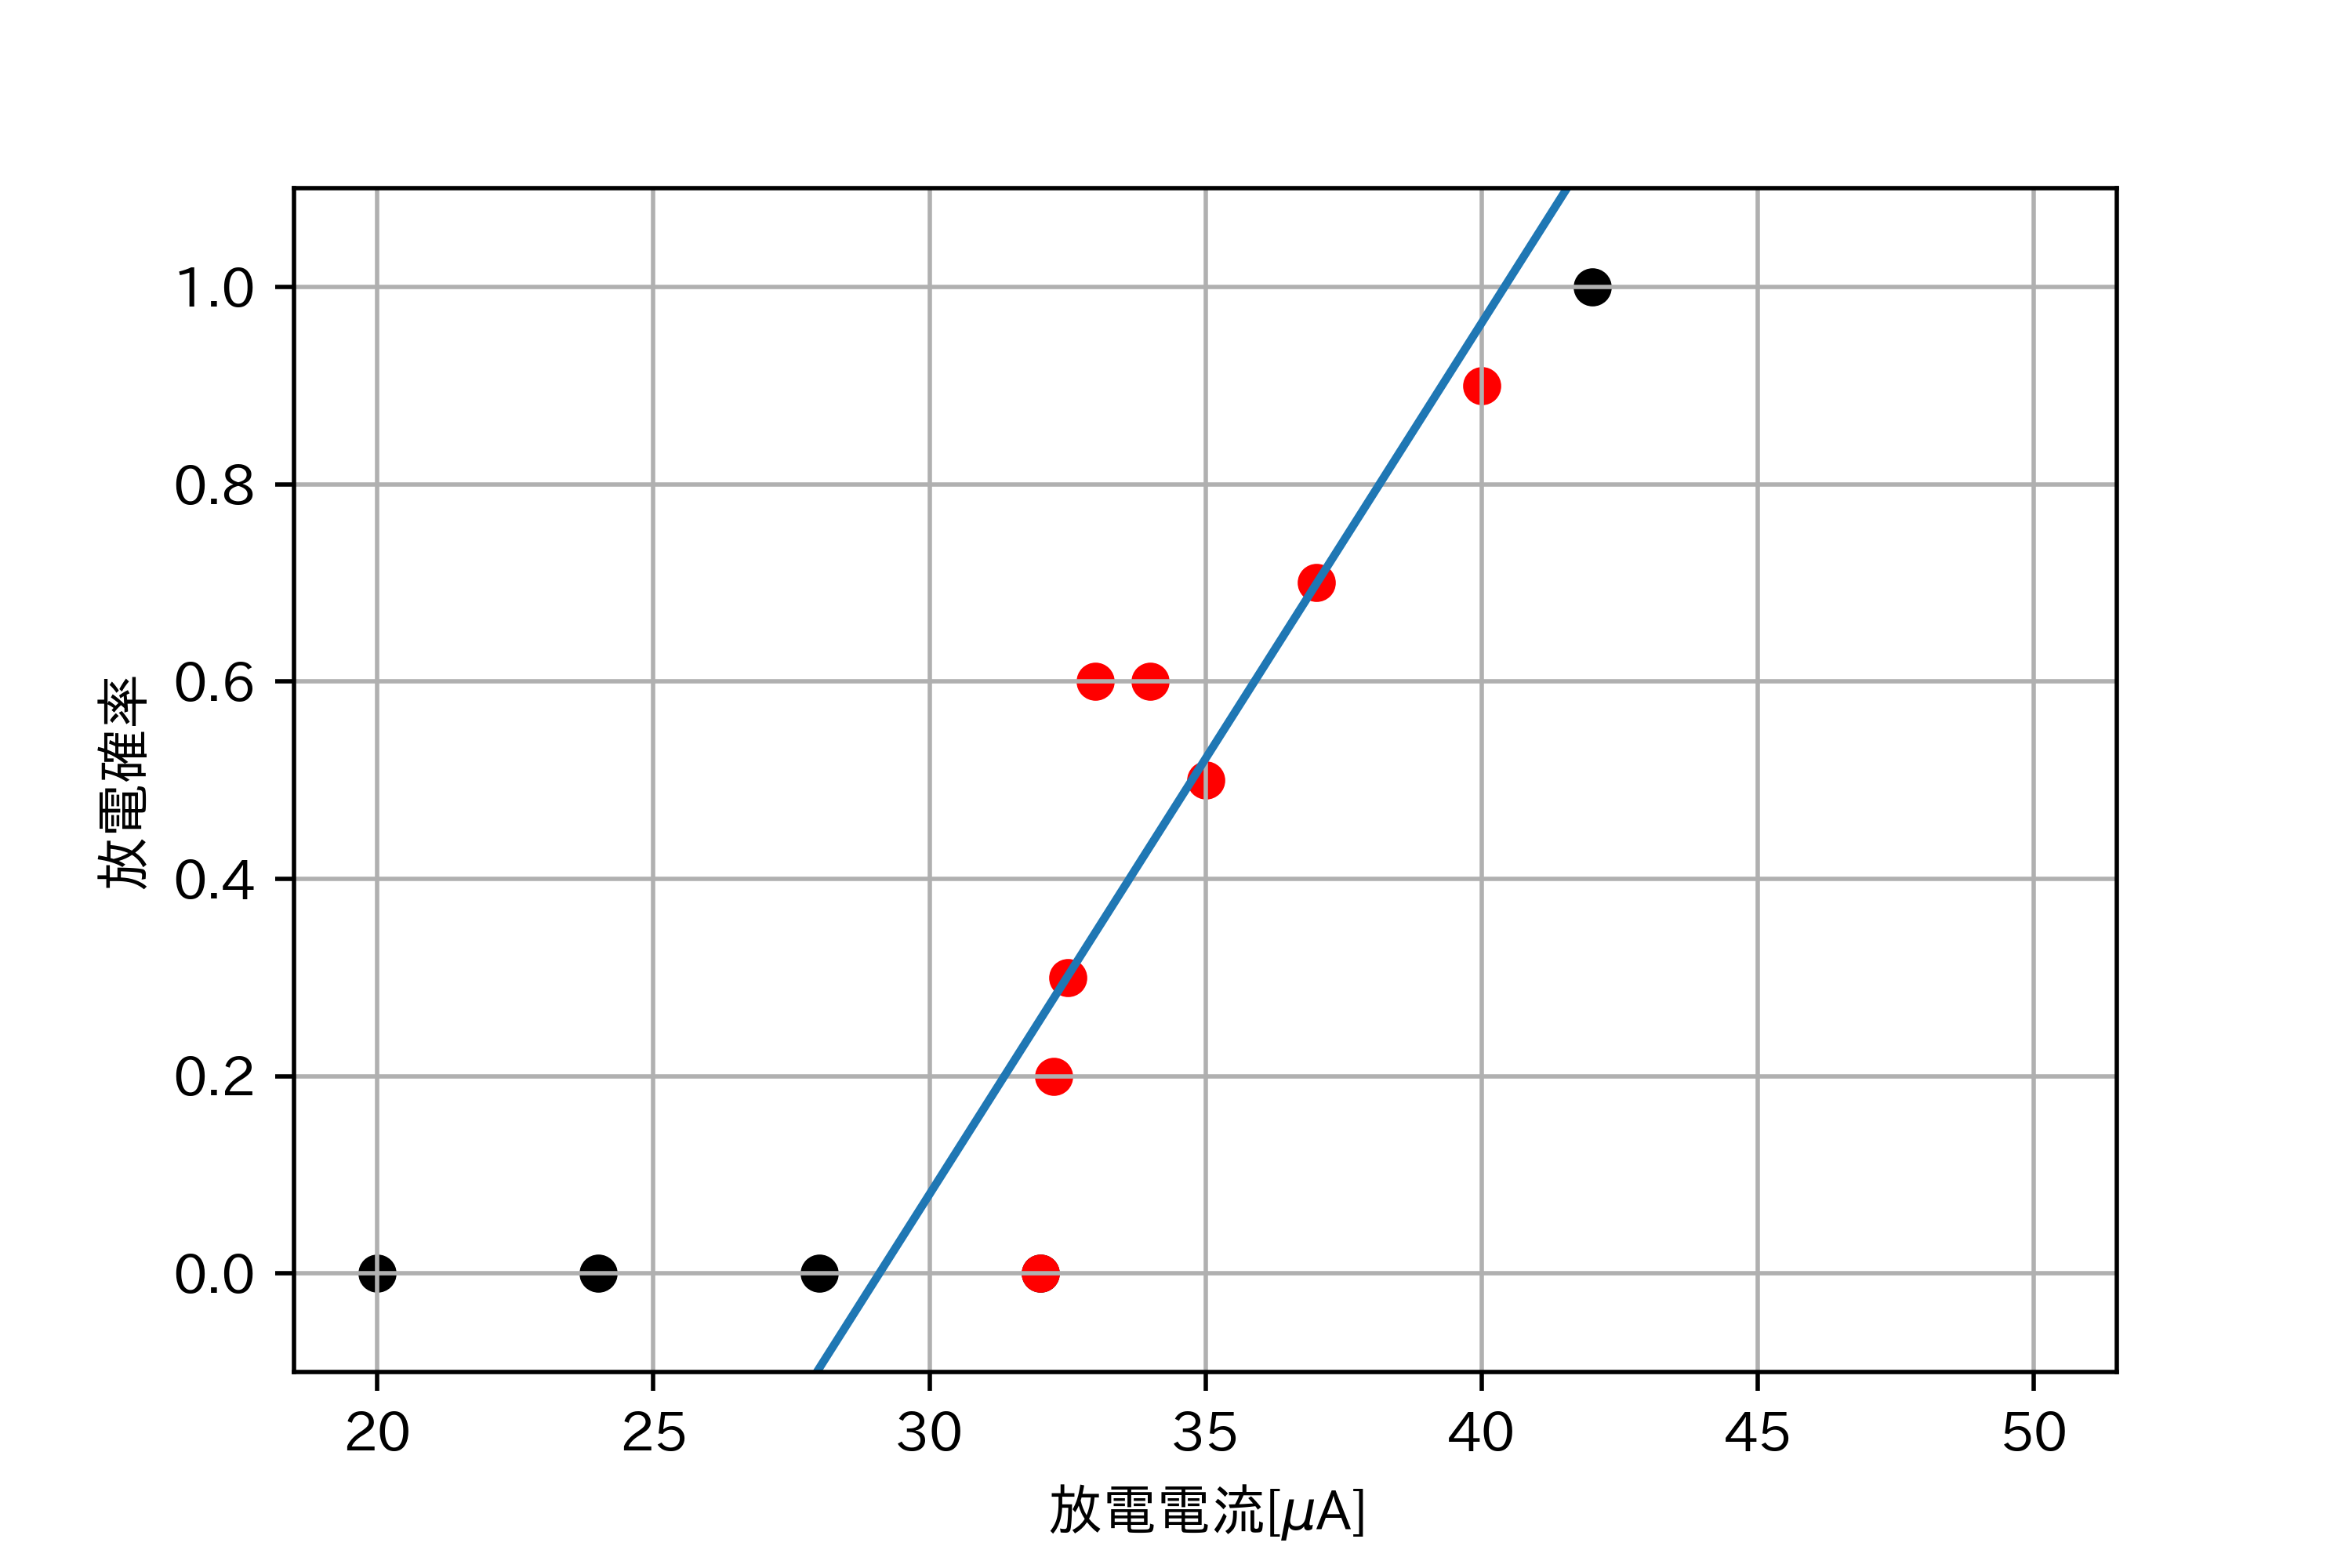
\includegraphics[scale = 0.5]{C42.png}
\caption{補間法による負極性の50\%火花電圧測定}
\end{center}
\end{figure}
50\% 電圧は48kV
\subsection*{D. 高電圧の測定}

\subsubsection*{D1. 非接触高電圧測定器による交流電圧波形の測定}

以下のグラフではCH2は分かりやすいように電圧値が全て50倍になっている。

\begin{figure}[H]
\begin{center}
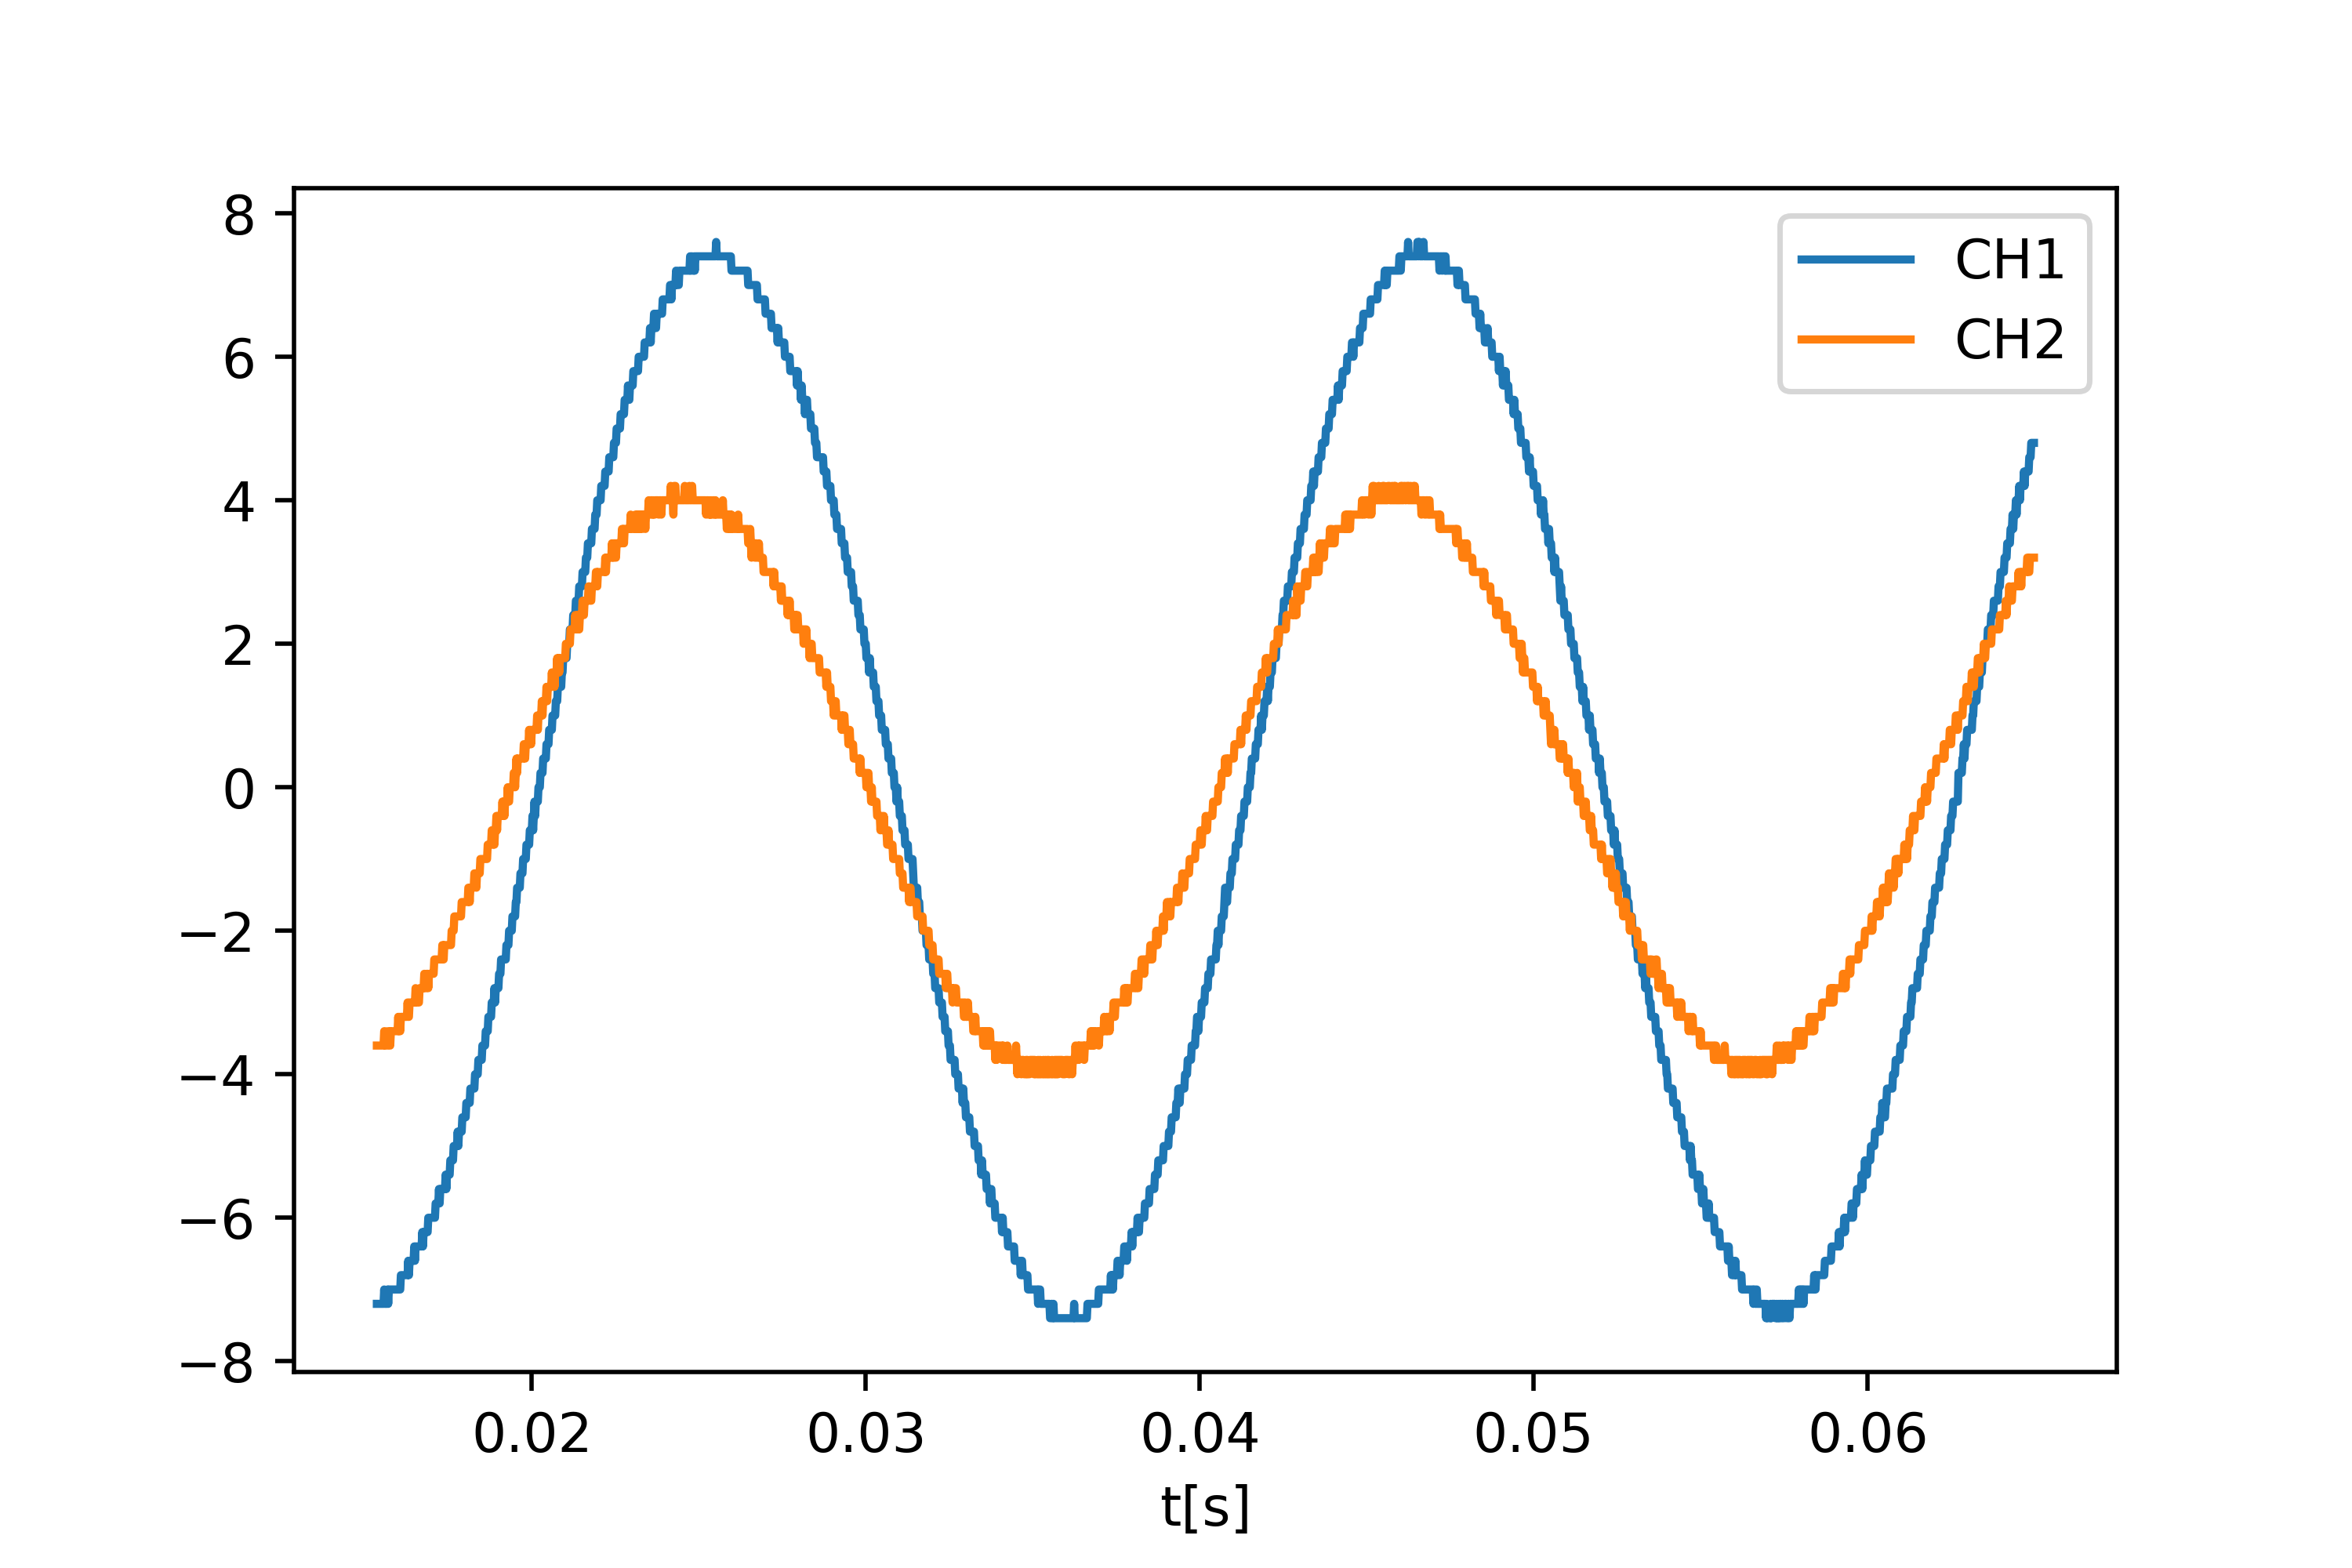
\includegraphics[scale = 0.5]{D11.png}
\caption{ポッケルスセンサによる交流波形測定(30mm)}
\end{center}
\end{figure}

\begin{figure}[H]
\begin{center}
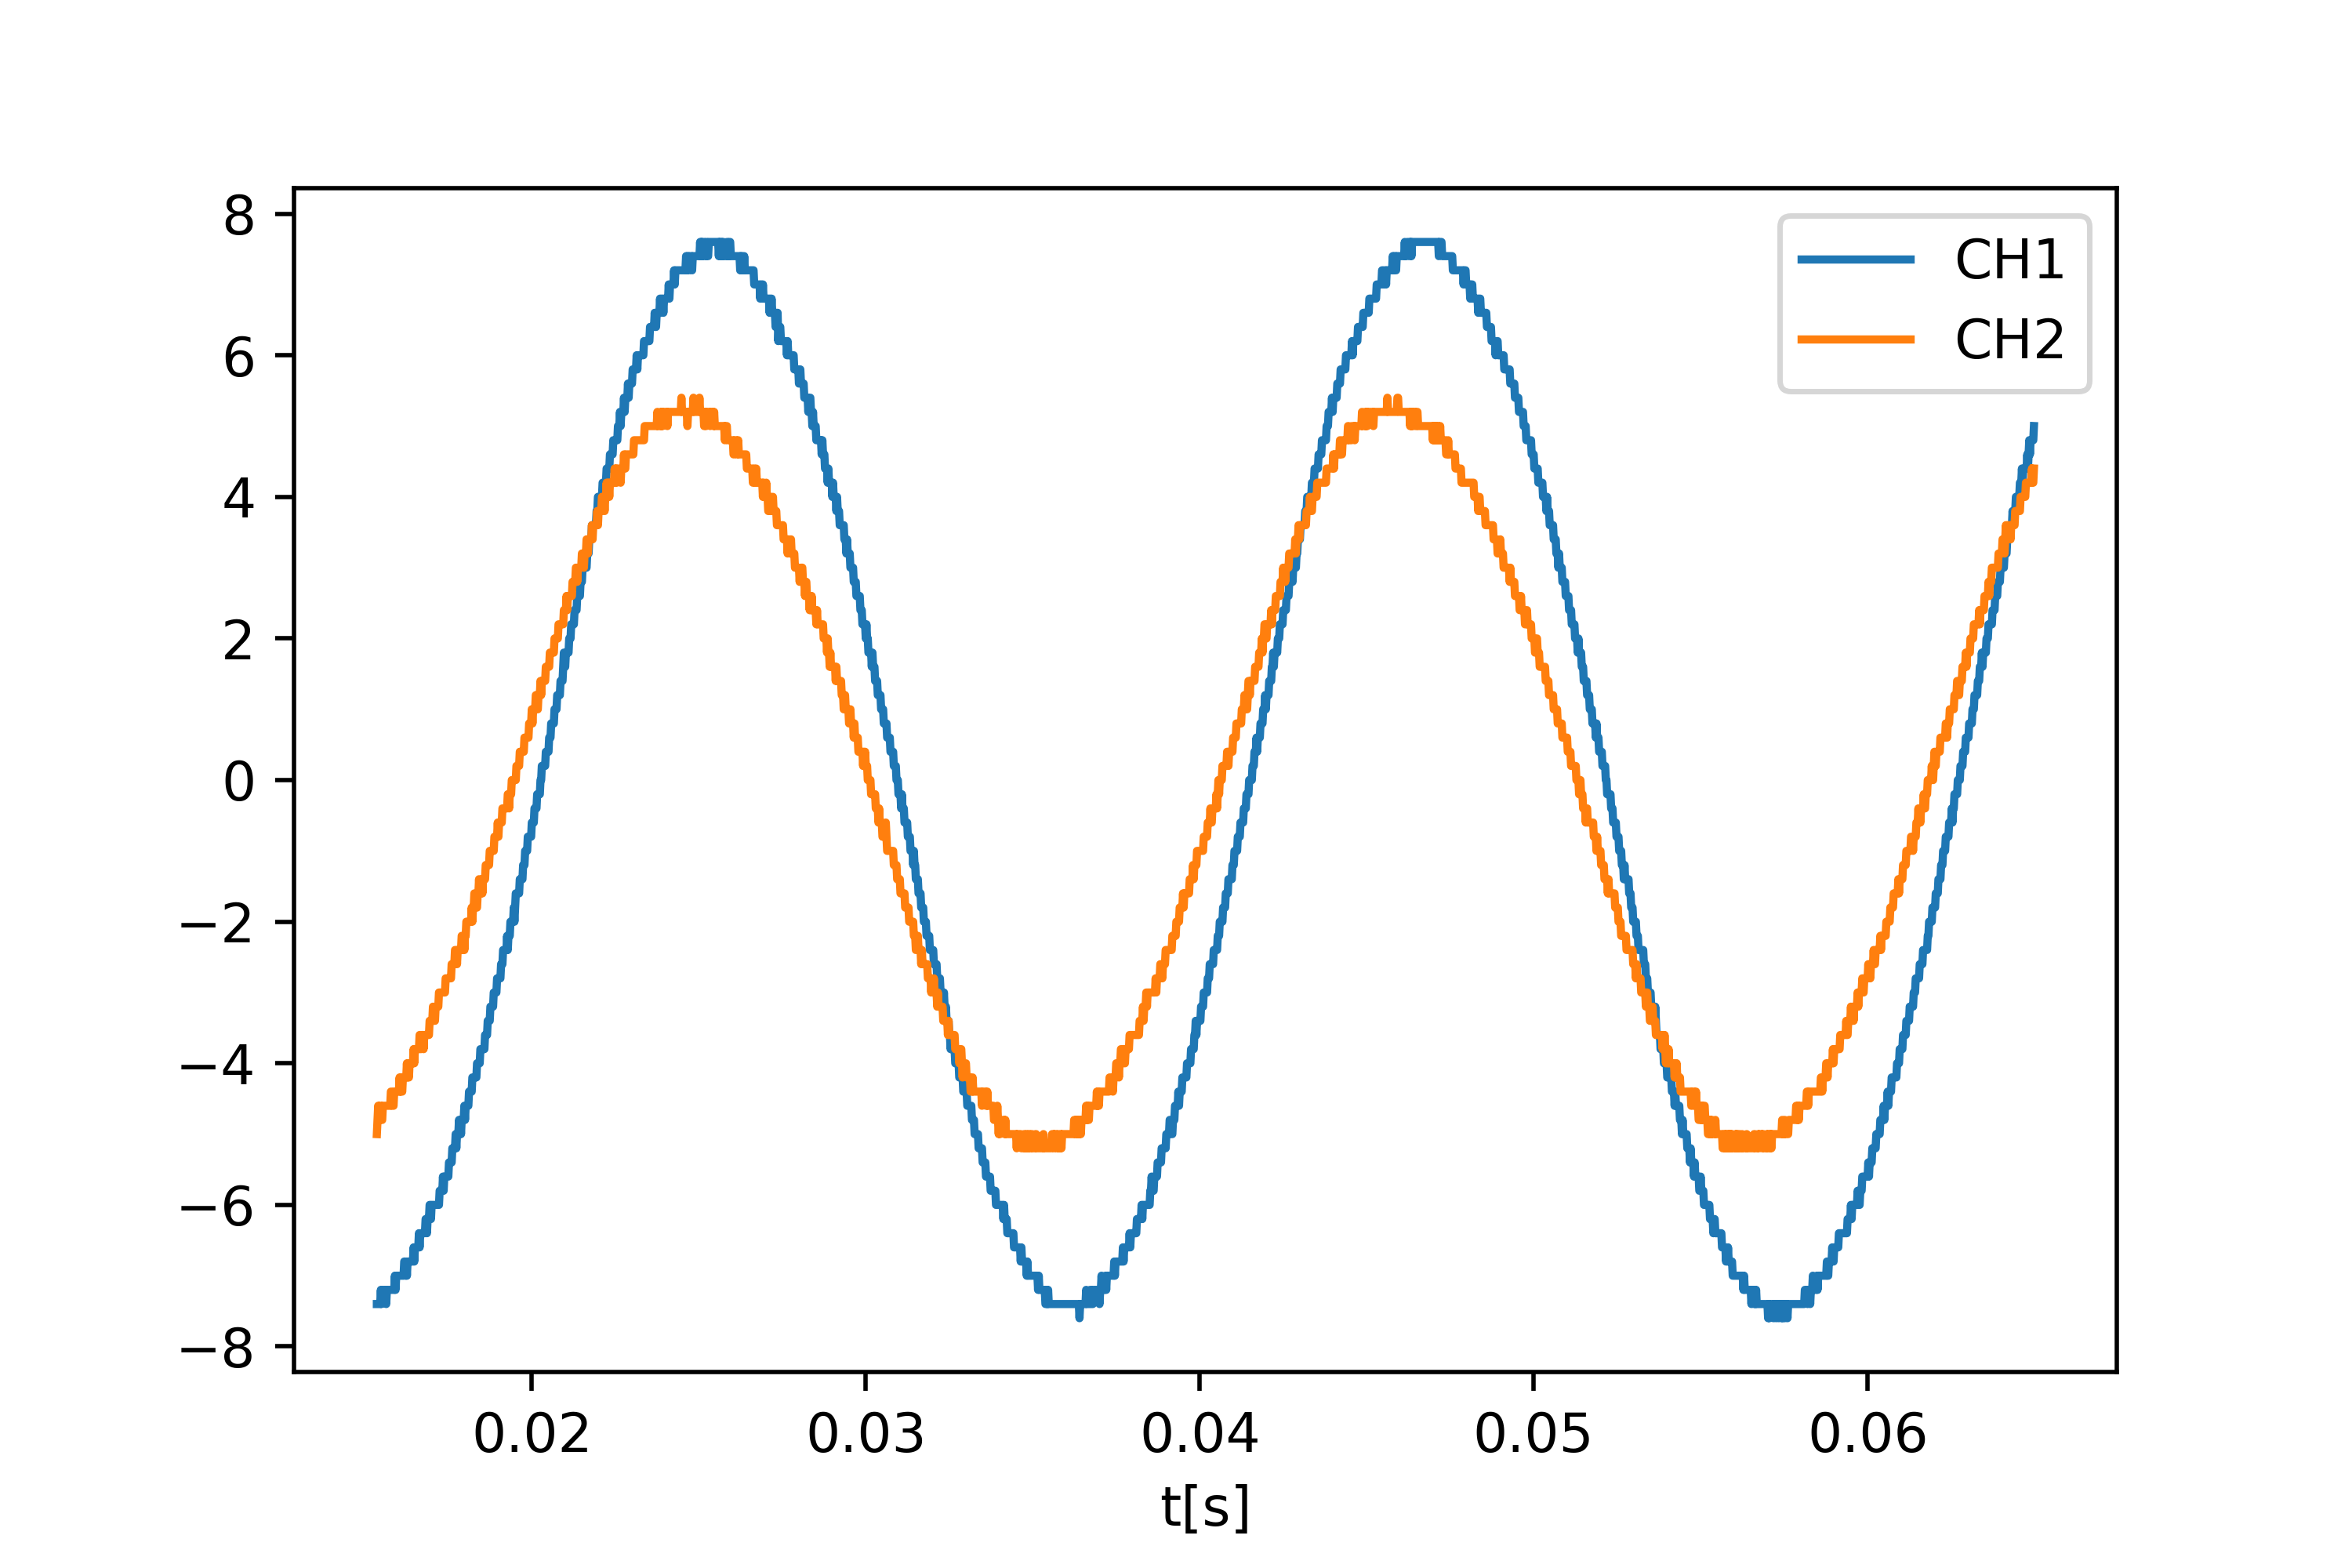
\includegraphics[scale = 0.5]{D12.png}
\caption{ポッケルスセンサによる交流波形測定(60mm)}
\end{center}
\end{figure}

\begin{figure}[H]
\begin{center}
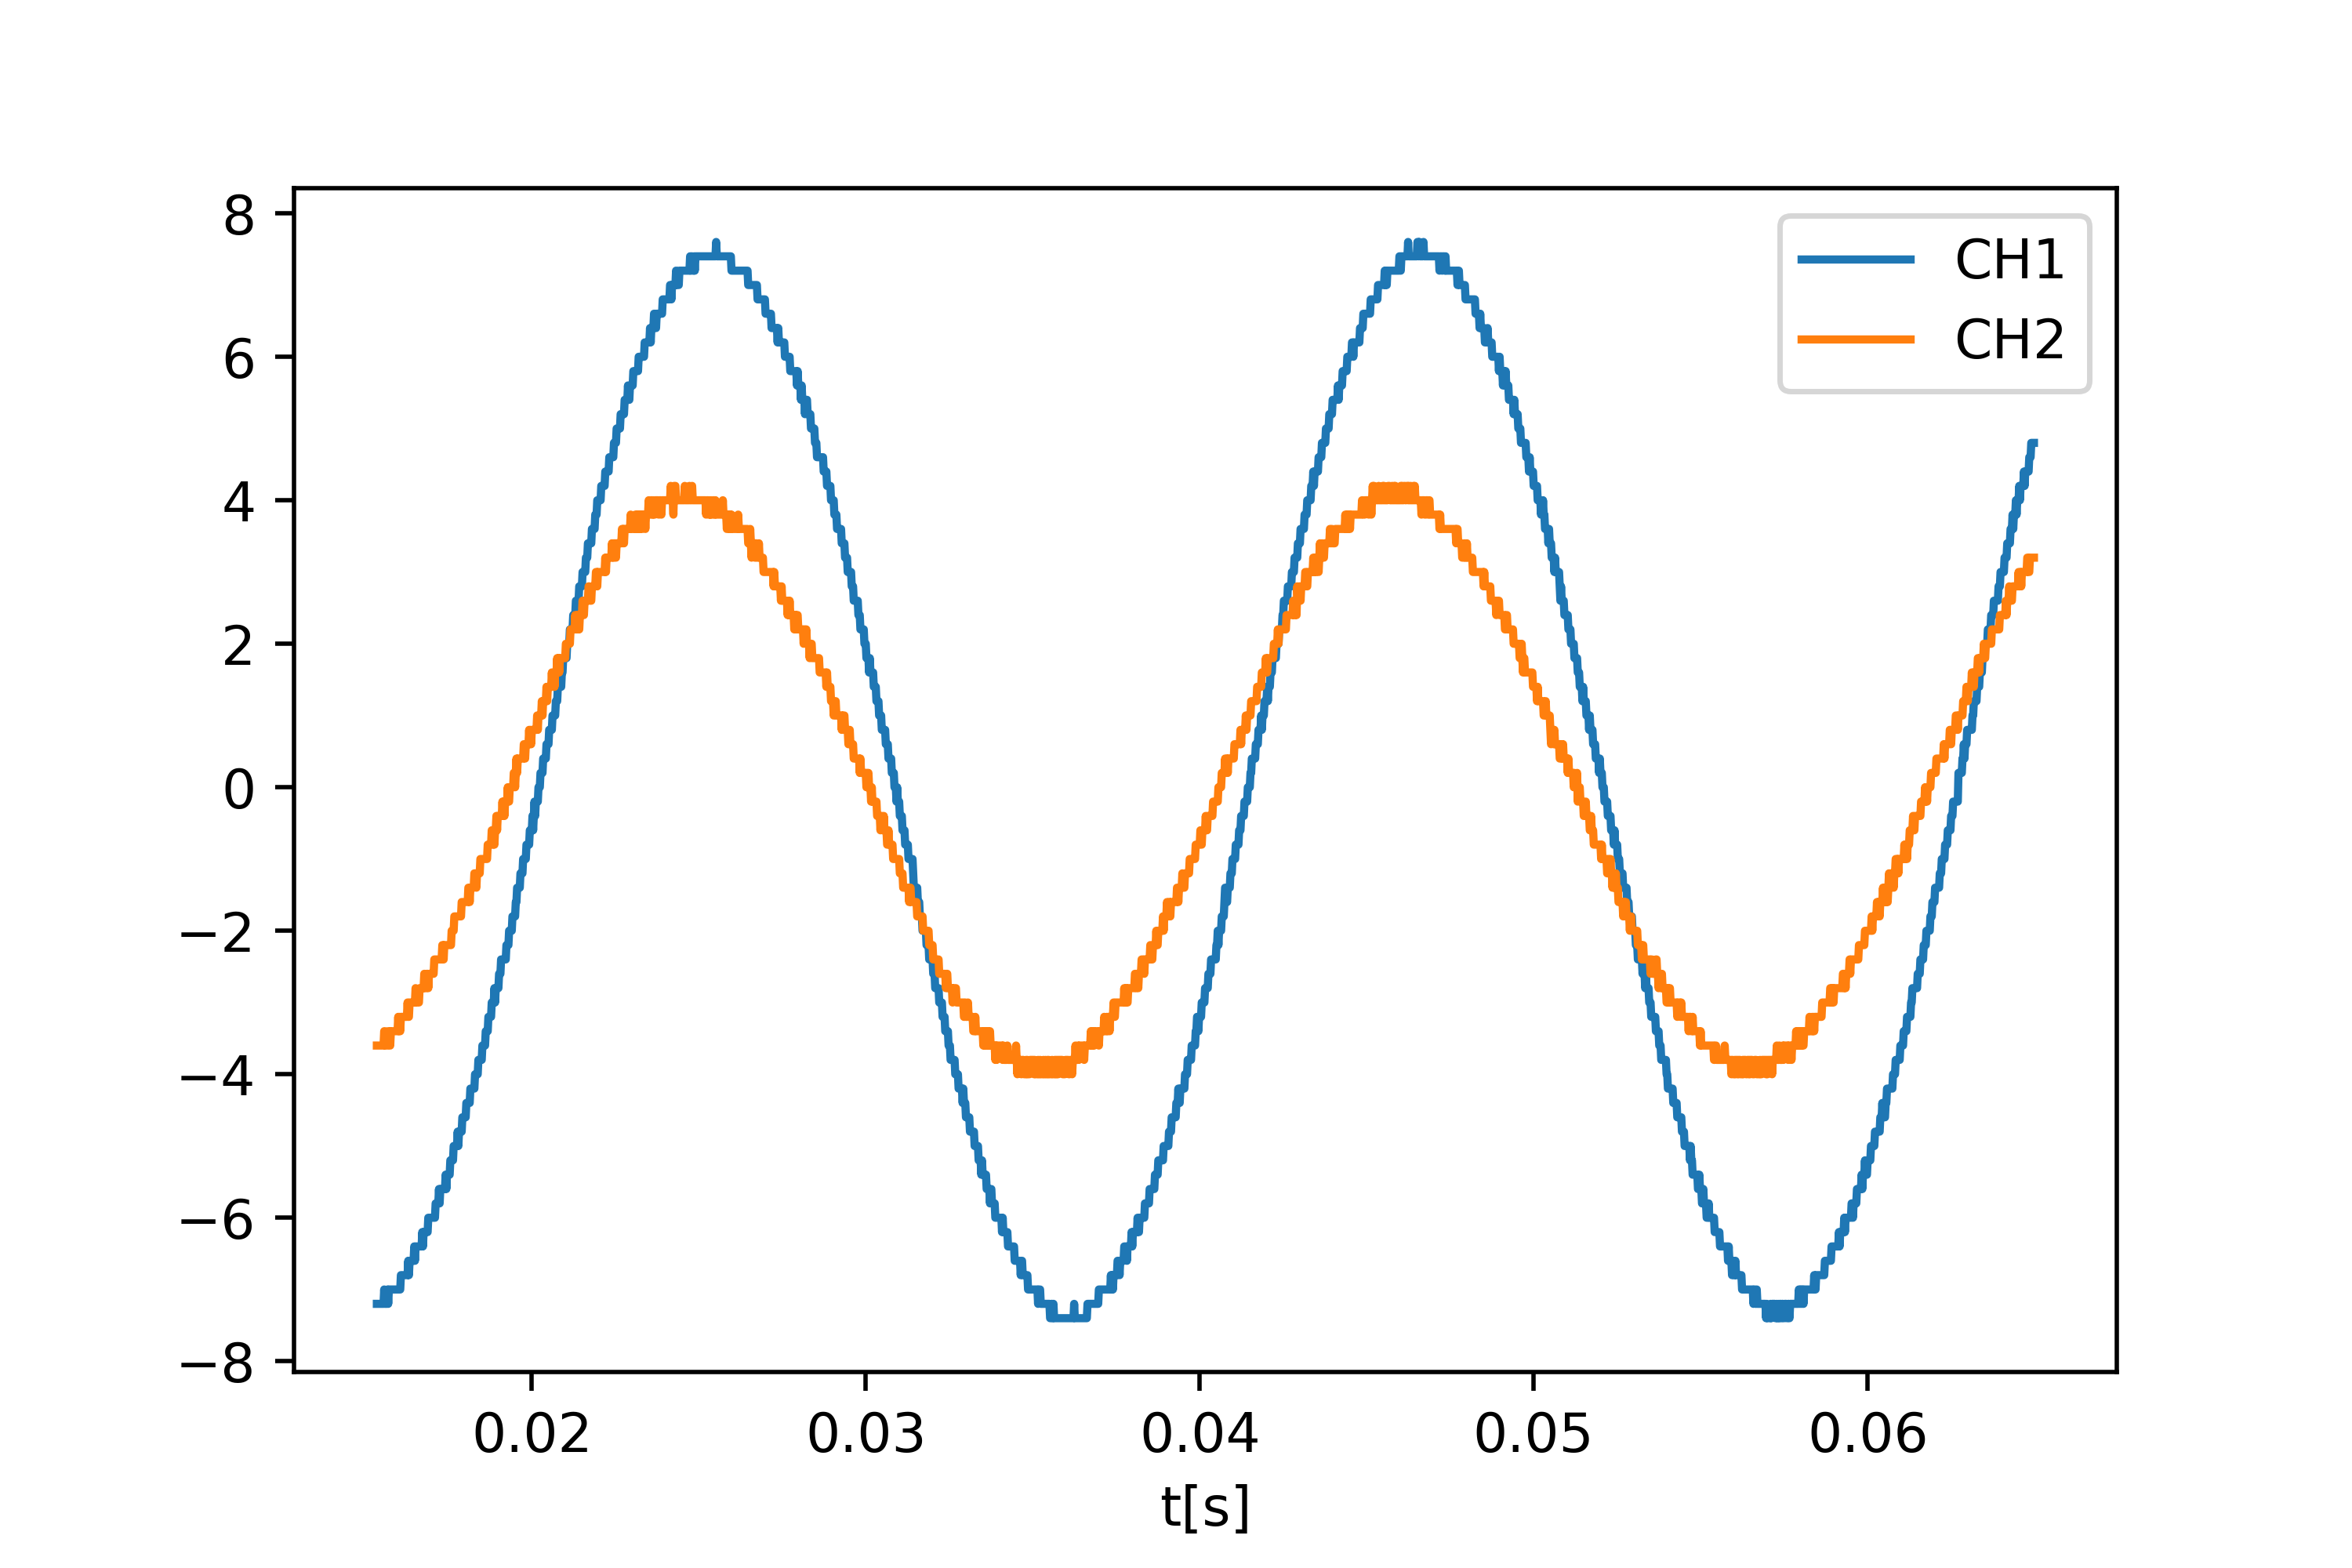
\includegraphics[scale = 0.5]{D13.png}
\caption{ポッケルスセンサによる交流波形測定(100mm)}
\end{center}
\end{figure}
\subsubsection*{D2. 非接触高電圧測定器による直流電圧の測定}

以下のグラフでもCH2は分かりやすいように電圧値が50倍になっている。
\begin{figure}[H]
\begin{center}
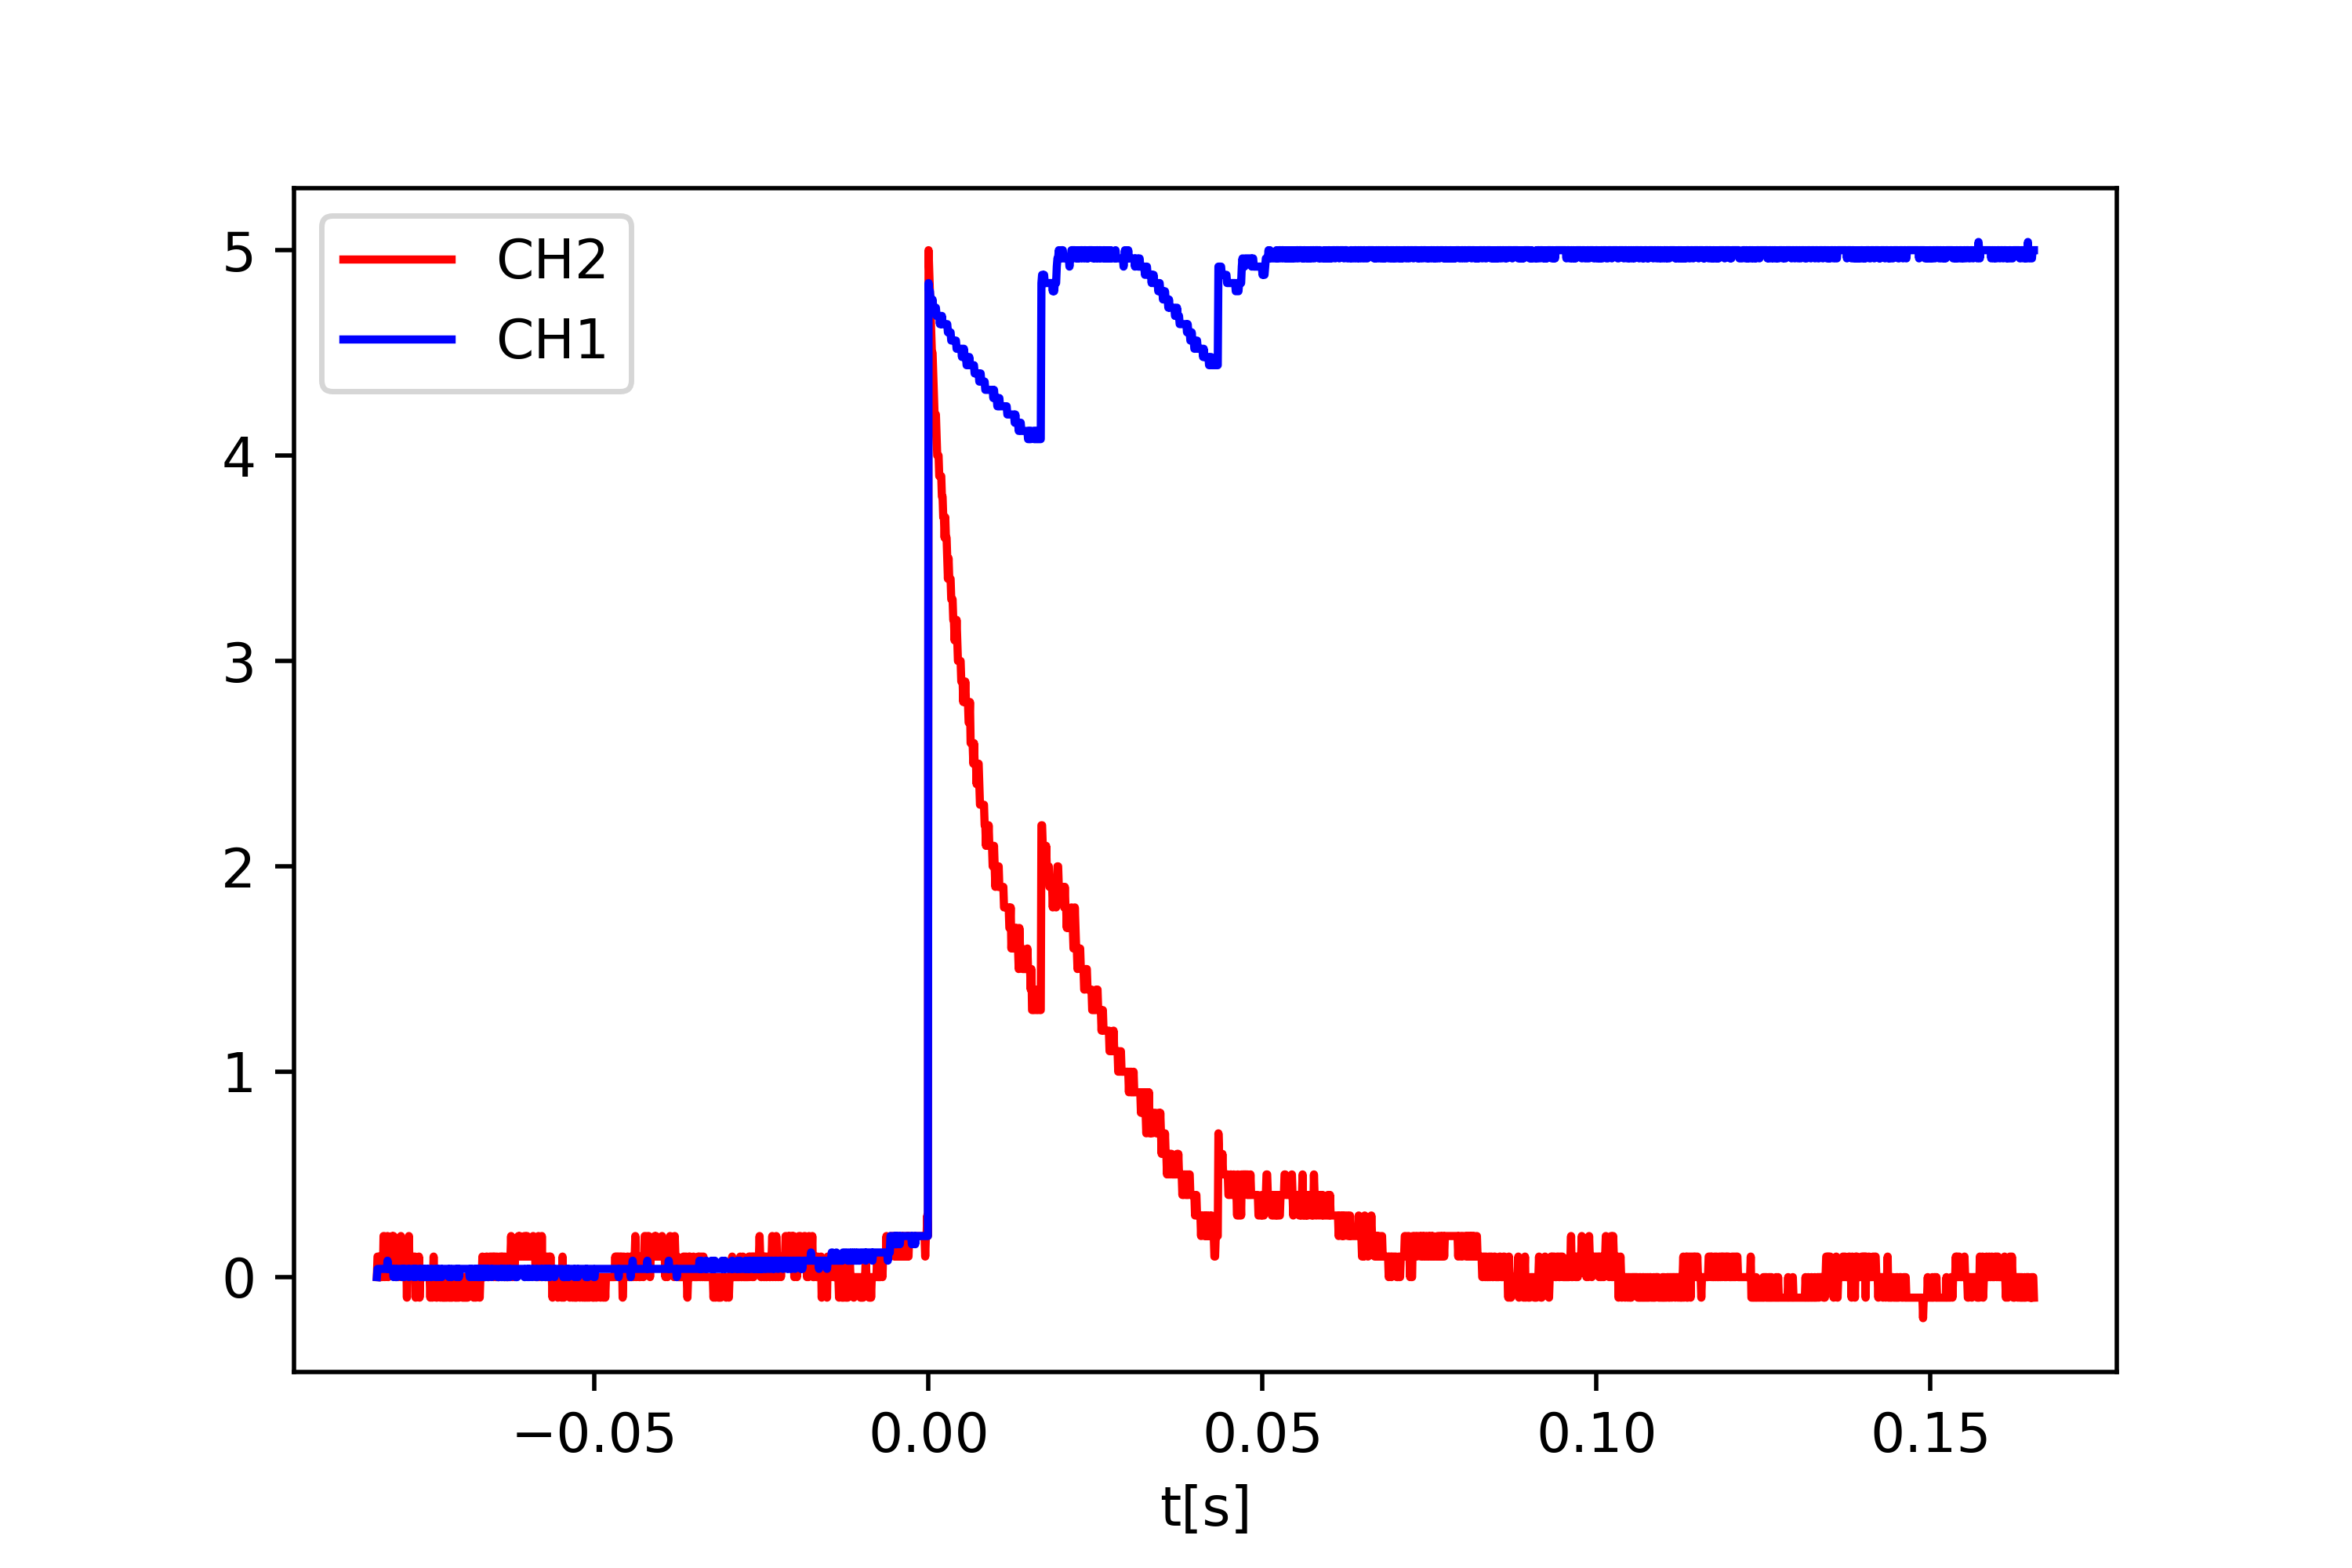
\includegraphics[scale = 0.5]{D2.png}
\caption{ポッケルスセンサによる直流電圧測定}
\end{center}
\end{figure}


\subsubsection*{D3. 分圧器の応答特性}
略

\section{検討・考察課題}
\subsection*{1.}
相対空気密度、湿度を測定しておく理由は、
気温を$t$[$^\circ$C]、気圧を$p$[mHg]、絶対湿度$h$[g/m$^{3}$]とすると火花電圧は相対空気密度$\delta = \frac{0.386\times p}{273+t}$、$k = 1 + 0.002\left(\frac{h}{\delta} - 8.5\right)$として、補正後の火花電圧$V_{s}$は$V_{s} = V_{n}\cdot \delta \cdot k$と表されるので、気温、気圧、湿度は電圧の校正に影響を与えるから。

\subsection*{2.}
50Hzの家庭用電圧をそのまま電源とし、試験用変圧器で変換すると、家庭用電圧は、様々なところで電力を消費され、試験用変圧器に歪んで届くので、補正する必要がある。

そこで、試験用変圧器の電源に歪みのない交流を発生させられる、正弦波発電機を使用している。


また、さらに補償リアクトルを挿入することで、遮断機がONになった時、充電電流が流れ続けるのを防ぐために、充電電流を補償リアクトルに流れる充電電流と逆位相の電流で打ち消すことができる(充電電流は電源電圧に対し$\pi /2$進み、補償リアクトルに流れる電流は$\pi /2$遅れている)。
\subsection*{3.}
針が正、平板が負の場合、

針と平板の距離は針の先端と平板との距離が最も近く、そこ以外は全て距離がかなり長くなるので、電子の流れは、平板から針の先端の間のみに集中し、局部的に強い電界が生じる。結果として、火花電圧は比較的低くなる。

一方で、針が負、平板が正の場合、

平板から見ると針周辺への距離はどこもさほど変わらない。そして電子の流れは、針から平板の方向になる。結果として平板の全体に電子の流れが分散するので放電は起こりにくくなり、結果として火花放電は正極性に比べて高くなる。
\subsection*{4.}

実験結果図6より、SF6中ではギャップ長1cmで62kV、2cmで113kVほどの火花電圧になっている。これは大気中での球球間火花放電圧が1cmで、32kV、2cmで59kVほどであることを考えるとその2倍程度になっており、SF6中では放電が起こりづらいと言える。

実際にSF6は高い絶縁性能を活かして、電力機器等で絶縁体として使用されている。
\subsection*{5.}
簡略化した放電時の回路図は以下
\begin{figure}[H]
\begin{center}
\begin{circuitikz}
\draw (0, 0) to [short, *-] (1.5, 0)
to [C = $\frac{C}{12}$] (1.5, 2)
to [resistor = $12r$] (1.5, 4)
to [short, -*] (0, 4)
;
\draw (1, 4) to [short, -o](2, 4);
\draw (2.05, 4) to [short](3, 4);
\draw (3, 4) to [short, o-](4, 4)
to [L = $L$](5, 4)
to [short] (6.5, 4)
to [resistor = $R_{s}$](8.5, 4)
to [short, -*](9, 4);
\draw (6, 4) to [short] (6, 3)
to [resistor = $R_{0}$, i = $i$] (6, 1)
to [short] (6, 0)
to [short] (1, 0);
\draw (6, 0) to [short, -*] (9, 0);
\draw (0, 0)to[open, v = $E$](0, 4);
\draw (9, 0)to[open, v = $V$](9, 4);
\end{circuitikz}
\end{center}
\caption{a}
\end{figure}

上の図より
\[L\frac{di}{dt} + (R_{0} + 12r)i + \frac{12}{C}\int idt = E\]

tで微分して
\[L\frac{d^{2}i}{dt^{2}} + (R_{0}+12r)\frac{di}{dt} + \frac{12}{C} = 0\]

これを解くと、
\[V(t) = \gamma E \{\exp{(-(\alpha - \beta)t})) - \exp{(-(\alpha + \beta)t})\}\]

ただし
\begin{equation*}
\alpha = \frac{R_{0} + 12r}{2L}, 
\beta = \frac{\sqrt{(R_{0}+12r)^{2}-4\frac{12L}{C}}}{2L}, 
\gamma = \frac{\alpha}{\beta}\frac{R_{0}}{R_{0}+12r}
\end{equation*}

これにC = $0.5\mu$F, r = 20$\Omega$, $R_{0} = 1.2\rm k \Omega$, $L = 530\mu$Hを代入して描画すると以下のグラフとなる。

\begin{figure}[H]
\begin{center}
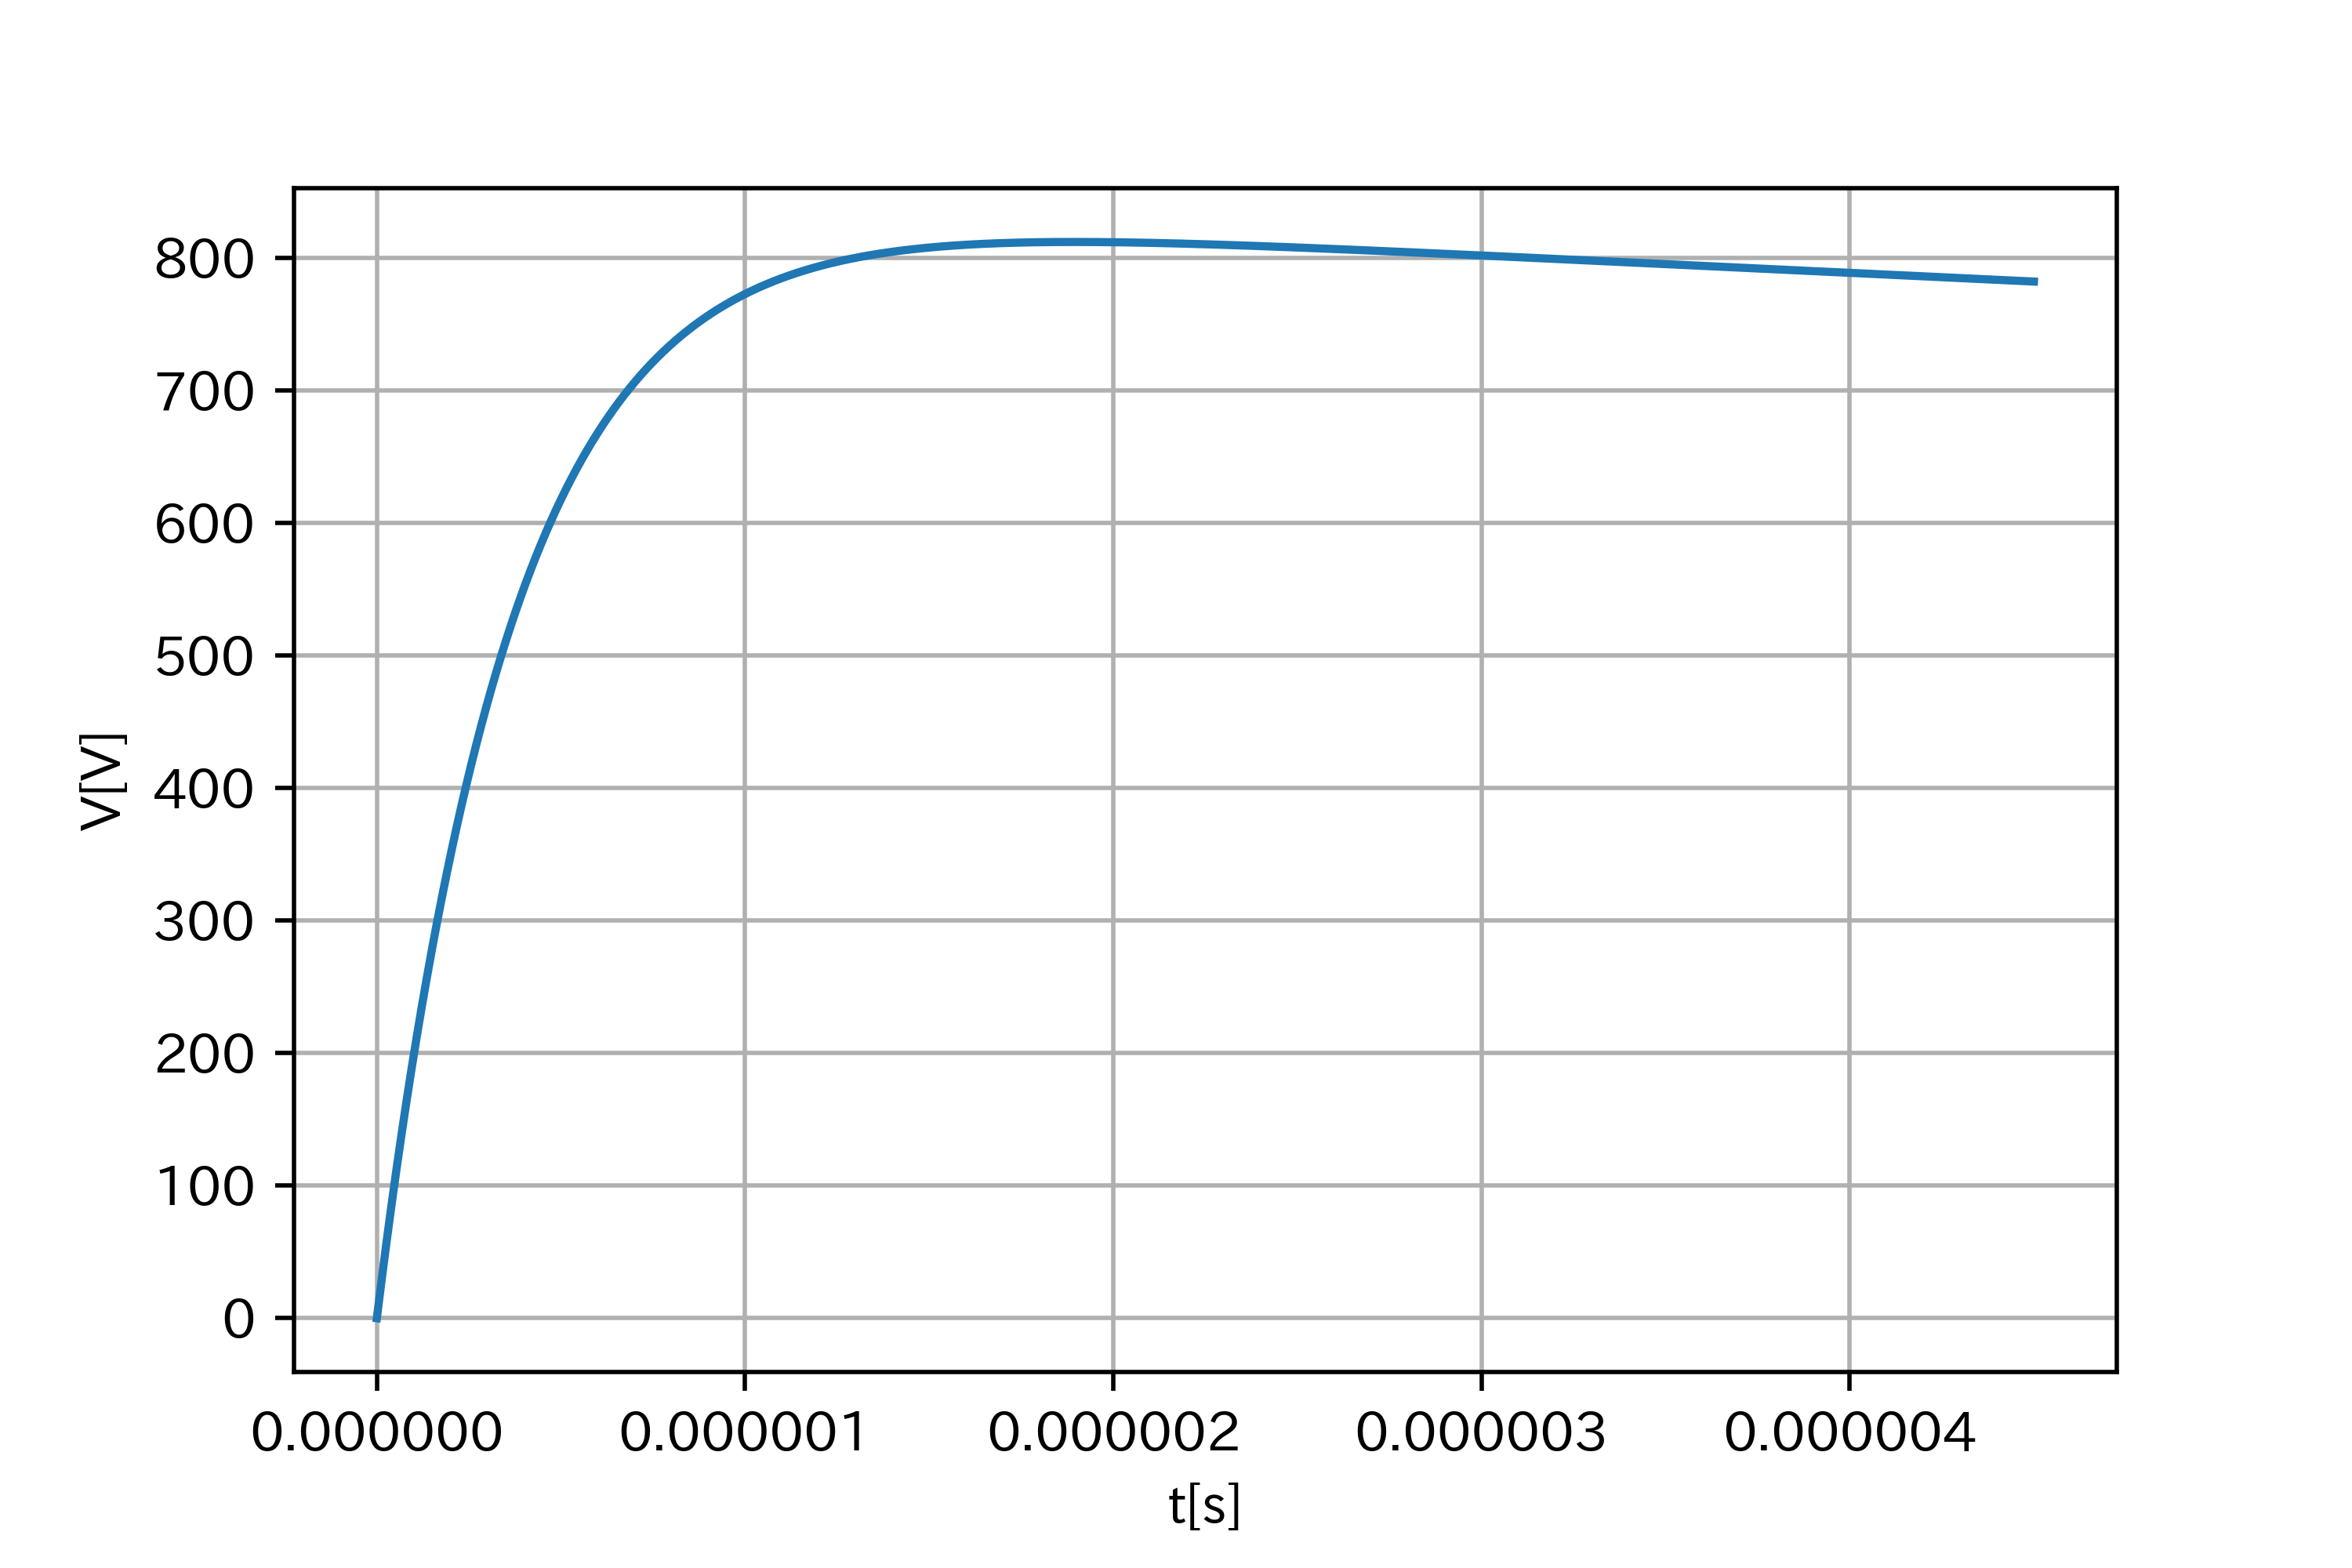
\includegraphics[scale = 0.5]{20_1.png}
\caption{インパルス電圧出力波形の理論値(1$\mu$s/div)}
\end{center}
\end{figure}
\begin{figure}[H]
\begin{center}
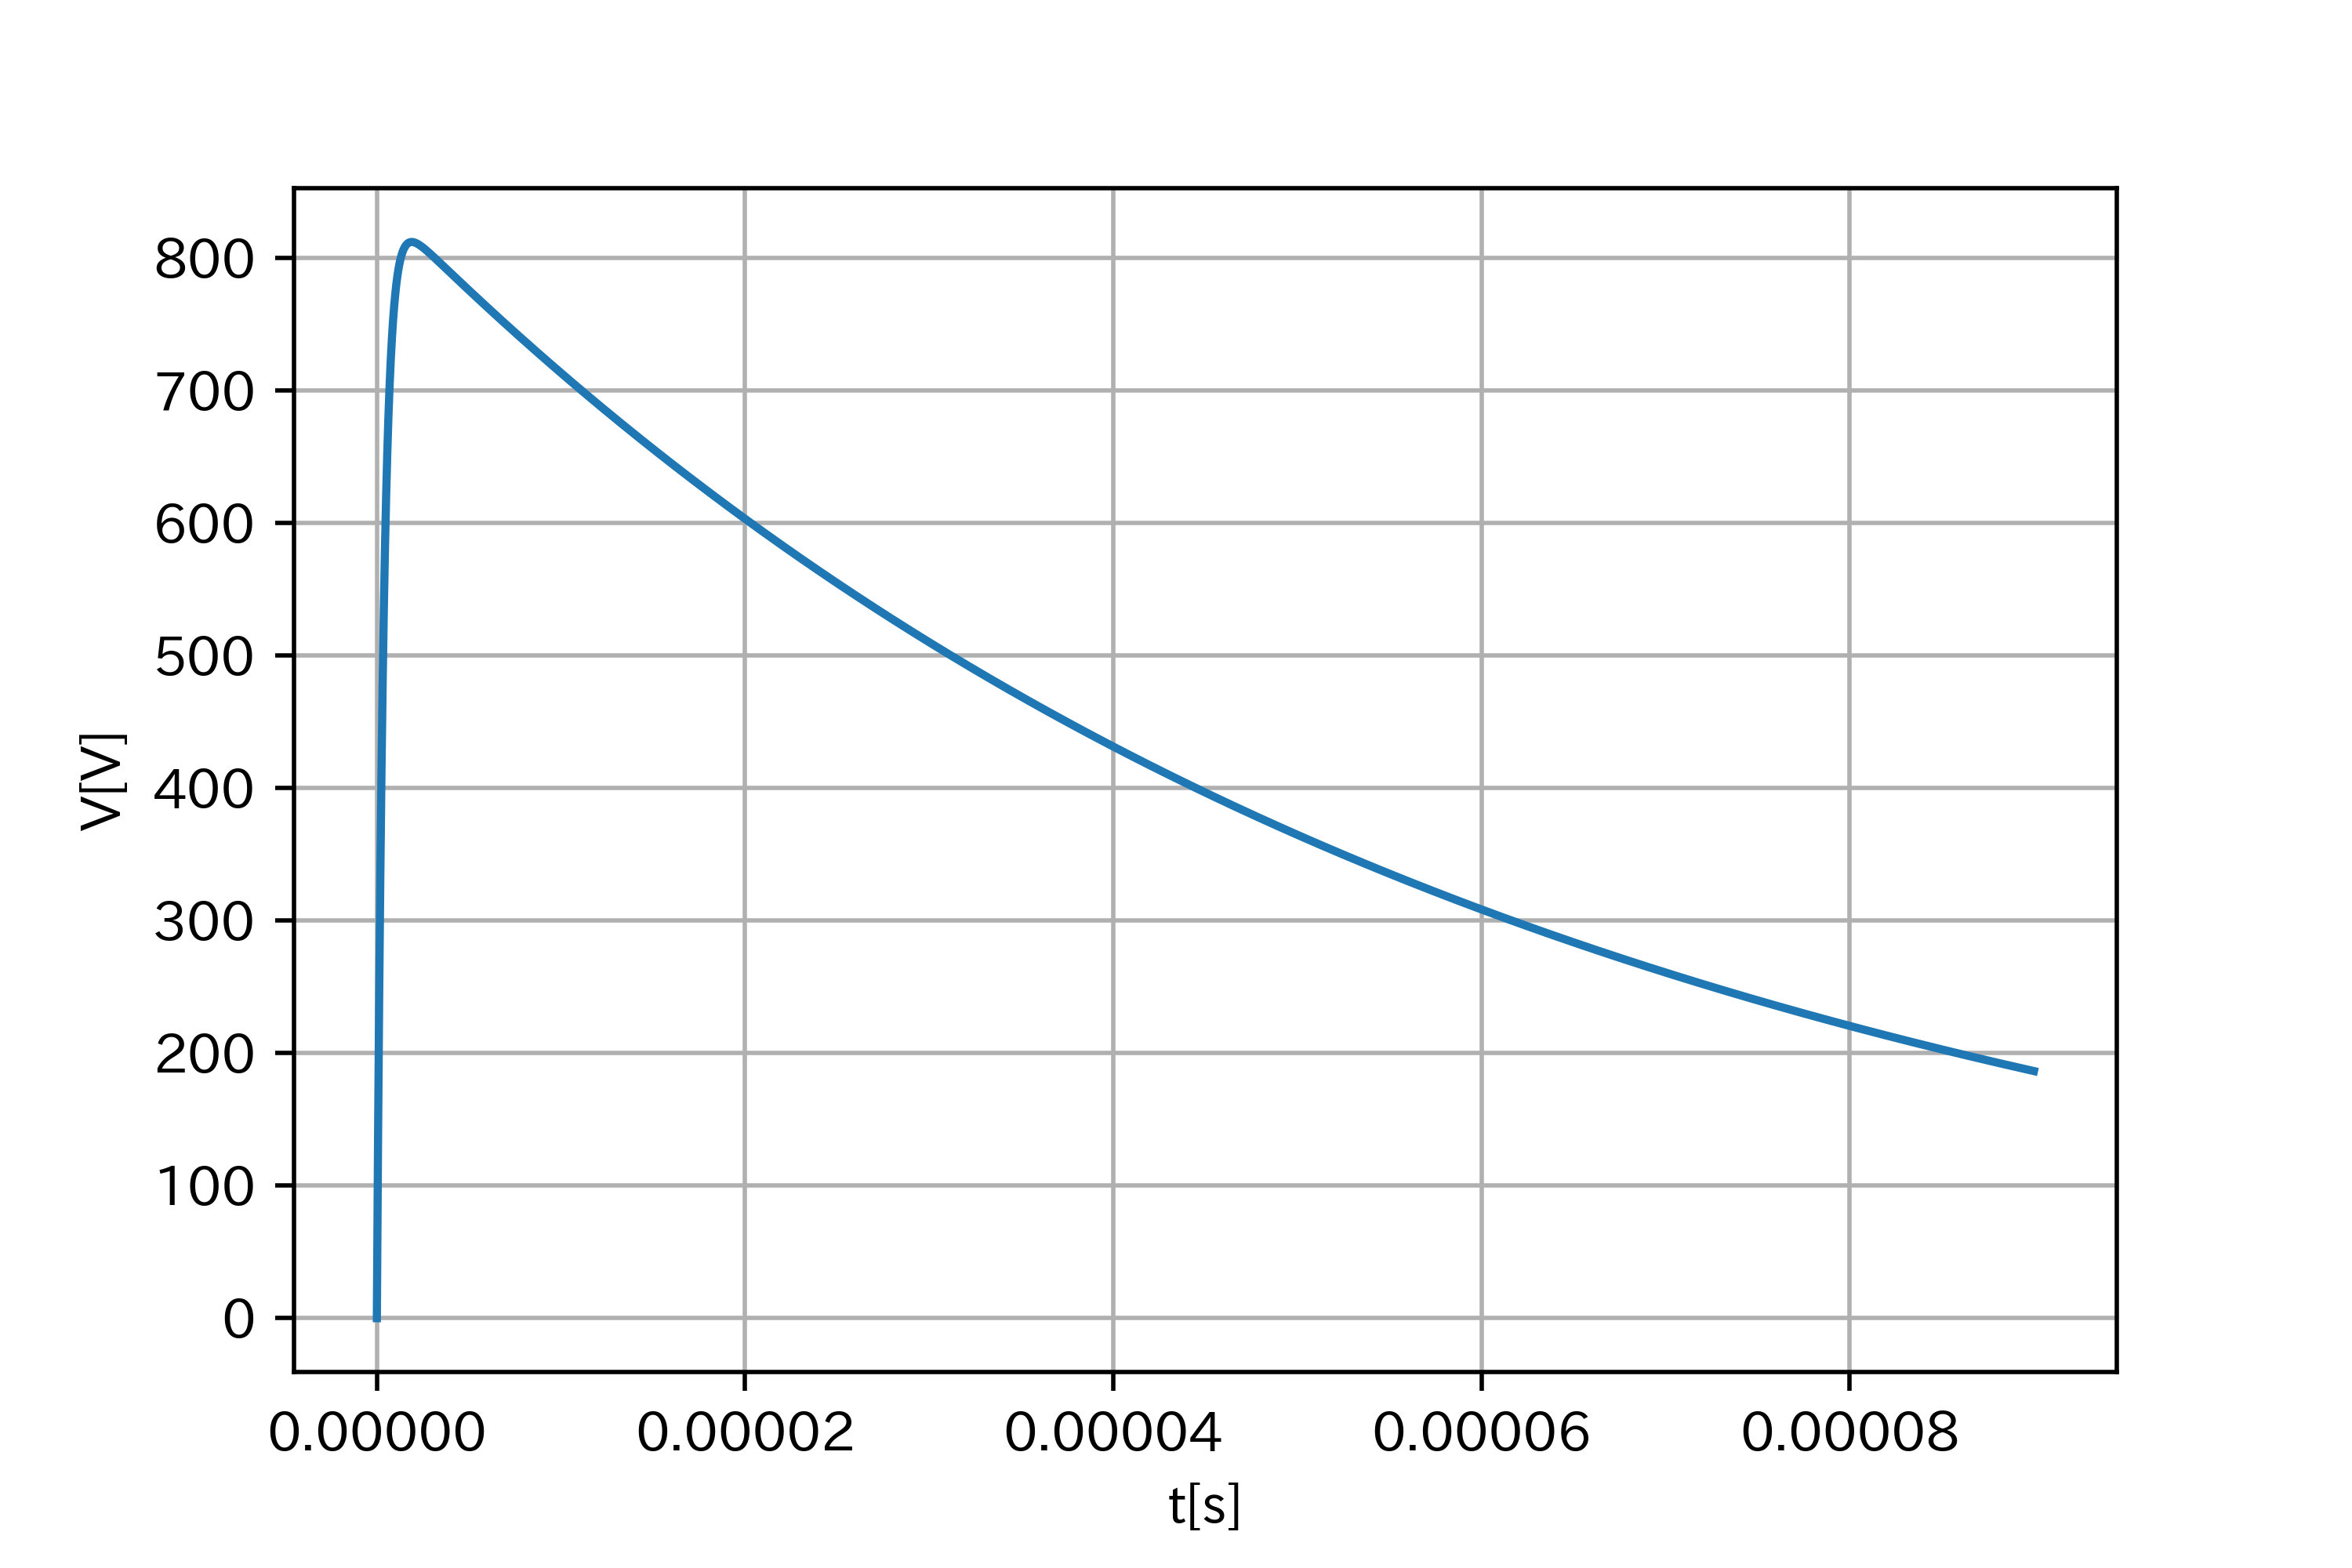
\includegraphics[scale = 0.5]{20_2.png}
\caption{インパルス電圧出力波形の理論値(20$\mu$s/div)}
\end{center}
\end{figure}

教科書の図と同じタイムスケールでプロットするとほぼ同じ形のグラフが得られていることがわかる。
\subsection*{6.}
図10より負極性のほうが10$\%$ほど火花電圧が小さくなっている。

球ギャップは平等電界なので、これは理論的に導かれる誤差ではなく、実験において生じる、温度や汚れに起因する誤差や確率の偏りが原因と考えられる。


棒平板ギャップについては、棒を針に見立てて、実験A3針-平板と同様に考えることができ、実際に負極性の方が火花電圧が大きくなっている。
\subsection*{7.}
・間接的に測定するので当然ではあるが、測定時に測定対象に与える擾乱が少ない。

・周囲からの電気的ノイズの影響を受けにくい。

・応答周波数範囲が広い。

がポッケルスセンサでの、直接的電圧、電界測定に対する利点となる。
\subsection*{8.}
浮遊容量が存在するので、直流をかけると、電流が流れにくくなるから。

また、交流では交流電流から発生する電磁波を測定することで接触せずに測定ができるが、電流の流れない直流電圧ではその電磁波の測定は難しいから。




\section{参考文献}
[1]東京大学工学部:「電気電子情報実験・演習第二 テキスト第2分冊」, 2019.

[2]廣瀬明:「電気電子計測」, 数理工学社, 2003.

[3]日高邦彦:「高電圧工学」, 数理工学社, 2013.

[4]河野照哉:「高電圧工学」, 朝倉書店, 1994.

[5]安藤晃, 犬竹正明:「高電圧工学」, 朝倉書店, 2006.
\end{document}